\documentclass[12pt, titlepage]{scrartcl}
\usepackage[ngerman]{babel}
\usepackage[ansinew]{inputenc}
\usepackage{color}
\usepackage[a4paper, lmargin={2.5cm}, rmargin={2cm}, tmargin={2.5cm}, bmargin={2.5cm}]{geometry}
\usepackage{amssymb}
\usepackage{amsthm}
\usepackage{graphicx}
\usepackage{subcaption}
\usepackage{booktabs}
\usepackage{float}
\usepackage{array}
\usepackage{adjustbox}
\usepackage{longtable}
\usepackage{booktabs}
\usepackage{helvet}
\usepackage{scrpage2}
\usepackage{wrapfig}
\usepackage{titlesec}
\usepackage{hyperref}
\renewcommand{\familydefault}{\sfdefault}
\renewcommand{\arraystretch}{1.2}
\pagestyle{scrheadings}
\clearscrheadfoot
\ofoot{\pagemark}
\ifoot{RBSG - Enhanced Wars}
\cfoot{Gruppe G}
\ohead{
\includegraphics[width=0.12\textwidth]{images/Logo.png}}
\ihead{Projektdokumentation}
\chead{Release \RN{3}}
\newcommand{\RN}[1]{%
	\textup{\uppercase\expandafter{\romannumeral#1}}%
}
\newcommand{\Abb}[1]{%
	Abb.\ \ref{#1}%
}
\titleclass{\subsubsubsection}{straight}[\subsection]
\newcounter{subsubsubsection}[subsubsection]
\renewcommand\thesubsubsubsection{\thesubsubsection.\arabic{subsubsubsection}}
\renewcommand\theparagraph{\thesubsubsubsection.\arabic{paragraph}}
\titleformat{\subsubsubsection}{\normalfont\normalsize\bfseries}{\thesubsubsubsection}{1em}{}
\titlespacing*{\subsubsubsection}{0pt}{3.25ex plus 1ex minus .2ex}{1.5ex plus .2ex}
\makeatletter
\renewcommand\paragraph{\@startsection{paragraph}{5}{\z@}%
  {3.25ex \@plus1ex \@minus.2ex}%
  {-1em}%
  {\normalfont\normalsize\bfseries}}
\renewcommand\subparagraph{\@startsection{subparagraph}{6}{\parindent}%
  {3.25ex \@plus1ex \@minus .2ex}%
  {-1em}%
  {\normalfont\normalsize\bfseries}}
\def\toclevel@subsubsubsection{4}
\def\toclevel@paragraph{5}
\def\toclevel@paragraph{6}
\def\l@subsubsubsection{\@dottedtocline{4}{7em}{4em}}
\def\l@paragraph{\@dottedtocline{5}{10em}{5em}}
\def\l@subparagraph{\@dottedtocline{6}{14em}{6em}}
\makeatother
\setcounter{secnumdepth}{4}
\setcounter{tocdepth}{4}
\begin{document}
    \begin{titlepage}
		\centering
		{\scshape\LARGE Projektdokumentation \par}
		\vspace{0.75cm}
		{\bfseries\Huge Release \RN{3}\par}
		\vspace{0.75cm}
		{\scshape\Large Universit\"at Kassel \par}
		{\scshape\Large Software Engineering \RN{1} SS 19\par}
		\vspace{0.5cm}
		{\bfseries\LARGE Projekt: Rundenbasiertes Strategiespiel \par}
		{\bfseries\LARGE RBSG - Enhanced Wars\par}
		\vspace{0.5cm}
		{\scshape\Large Gruppe G\par}
		\vspace{1.5cm}
		{
\includegraphics[width=1\textwidth]{images/Logo.png}\par}
		\vspace{0.5cm}
		{\scshape\Large Scrum Master: Jan M"uller\par}
		{\scshape\Large Product Owner: Keanu St"uckrad\par}
		\vspace{0.75cm}
		{\bfseries\Large 8.7.2019 - 4.8.2019\par}
	\end{titlepage}	
	\pagenumbering{arabic}
	\setcounter{page}{1}	
	\section{Vorwort}
    	Das Release \RN{3} von Gruppe G des Projekts RBSG, ein rundenbasiertes Strategiespiel, soll im Rahmen des Moduls \glqq Software Engineering \RN{1}\grqq\ im Fachbereich \glqq Software Engineering\grqq\ im Sommersemester 2019 mit dieser Dokumentation festgehalten werden.
    	\vspace{0.3cm} \newline
        Das Vorgehen in diesem Modul ist so gegliedert, dass es vier Releases mit jeweils zwei Sprints "uber vier Monate gibt. Das Projekt begann am 13.5.2019 und wird bis zum 1.9.2019 laufen. Ein Client f"ur einen Klon vom Klassiker \glqq Advanced Wars\grqq\ soll entwickelt werden. Dabei ist das Team "uber die vier Releases immer in einen Scrum Master, einen Product Owner und mehrere Developer eingeteilt.
        \vspace{0.3cm} \newline
        Die Dokumentation wird eine Einleitung in das Release, danach die Zusammenfassung der beiden Sprints und eine abschlie"sende Releaseanalyse enthalten. In der Einleitung sollen die Anforderungen des Kunden, der letzte Standpunkt und die neuen MockUps erl"autert werden. In den Sprintdokumentationen wird jeweils kurz das Ziel dargelegt und darauf sollen alle User Stories, Tasks oder Bugs aufgelistet werden. Am Ende wird es immer eine Zeit\"ubersicht mit einer Analyse des Sprints geben. Das letzte Kapitel mit der Releaseanalyse wird aufzeigen, ob das Resultat den Anforderungen entspricht und ob das Team effektiv arbeitete.
    \newpage
    \tableofcontents
    \newpage
    \section{Release \RN{3}}
        Das Release \RN{3} erstreckte sich "uber die vier Wochen vom 8.7.2019 bis zum 4.8.2019. Die zwei Sprints gingen vom 8.7.2019 bis zum 21.7.2019 und vom 22.7.2019 bis zum 4.8.2019.
        \vspace{0.1cm} \newline
        Das Team war in diesem Release wie gefolgt aufgeteilt:
        \begin{itemize}
            \item Scrum Master:  \hspace{0.275cm} 
\includegraphics[width=0.05\textwidth]{images/avatars/jan.png} \ Jan M"uller
    		\item Product Owner:   \hspace{0.1cm} 
\includegraphics[width=0.05\textwidth]{images/avatars/keanu.png} \ Keanu St"uckrad
    		\item Developer:
    		\begin{enumerate}
    		    \item 
\includegraphics[width=0.05\textwidth]{images/avatars/georg.png} \ Georg Siebert
    		    \item 
\includegraphics[width=0.05\textwidth]{images/avatars/juri.png} \ Juri Lozowoj
    		    \item 
\includegraphics[width=0.05\textwidth]{images/avatars/omar.png} \ Omar Sood 
    		    \item 
\includegraphics[width=0.05\textwidth]{images/avatars/tobias.png} \ Tobias Klipp
    		\end{enumerate}
        \end{itemize}
        \subsection{Releaseanforderungen}
            Folgende Mindestanforderungen wurden vereinbart:
            \begin{enumerate}
                \item Client: Waiting Room (Gamelobby)
                \begin{itemize}
                    \item Chatfunktion
                    \item Armeeauswahl
                    \item Senden eines Bereit-Signals
                \end{itemize}
                \item Client: Ingame
                \begin{itemize}
                    \item Bewegen und Angreifen von Einheiten
                    \item Minikarte
                    \item Chatfunktion
                    \item Anzeige aller Spieler
                    \item Anzeige der aktuellen Runde und Phase
                    \item Anzeige des Gewinners
 			\item Spiele verlassen
			\item Beobachtermodus
                \end{itemize}
                \item Client: Lobby
                \begin{itemize}
                    \item Spielbeitritt als Beobachter
                \end{itemize}
                \item Qualit"atssicherung
                \begin{itemize}
                    \item C0 Testabdeckung von 75\%
                \end{itemize}
            \end{enumerate}
        \subsection{Standpunkt des letzten Releases}
            Das Release \RN{2} erstreckte sich vom 10.6.2019 bis zum 7.7.2019. Nach dem 7.7. waren folgende Teile des Clients fertig gestellt:
            \begin{itemize}
                \item Login
                \begin{itemize}
                    \item[$\ast$] Anmelden
                    \item[$\ast$] Registrieren
                \end{itemize}
                \item Lobby
                \begin{itemize}
                    \item[$\ast$] Spiel erstellen/beitreten
                    \item[$\ast$] Anzeige der angemeldeten Spieler 
                    \item[$\ast$] Anzeige der aktiven Spiele
                    \item[$\ast$] Chatfunktion
                    \item[$\ast$] Ausloggen
                \end{itemize}
                \item Army Manager
                \begin{itemize}
                    \item[$\ast$] Konfigurieren eigener Armeen
                    \item[$\ast$] Speichern von Armeen lokal und auf dem Server
                \end{itemize}
                \item Waiting Room (Gamelobby)
                \begin{itemize}
                    \item[$\ast$] Chatfunktion
                    \item[$\ast$] Anzeige der beigetretenen Spieler 
                    \item[$\ast$] Zur"uck zur Lobby
                \end{itemize}
                \item Ingame
                \begin{itemize}
                    \item[$\ast$] Anzeige des initialen Spielgeschehens
                    \item[$\ast$] Zur"uck zur Lobby
                \end{itemize}
            \end{itemize}
            Weiterhin wurde bereits eine C0 Testabdeckung von mindestens 60\% erreicht.
            \subsubsection{Login}
                Im Login konnte der Nuzter sich anmelden oder registrieren (siehe Abbildung \ref{Login}). \\
                \begin{figure}[H] 
    				\centering
    				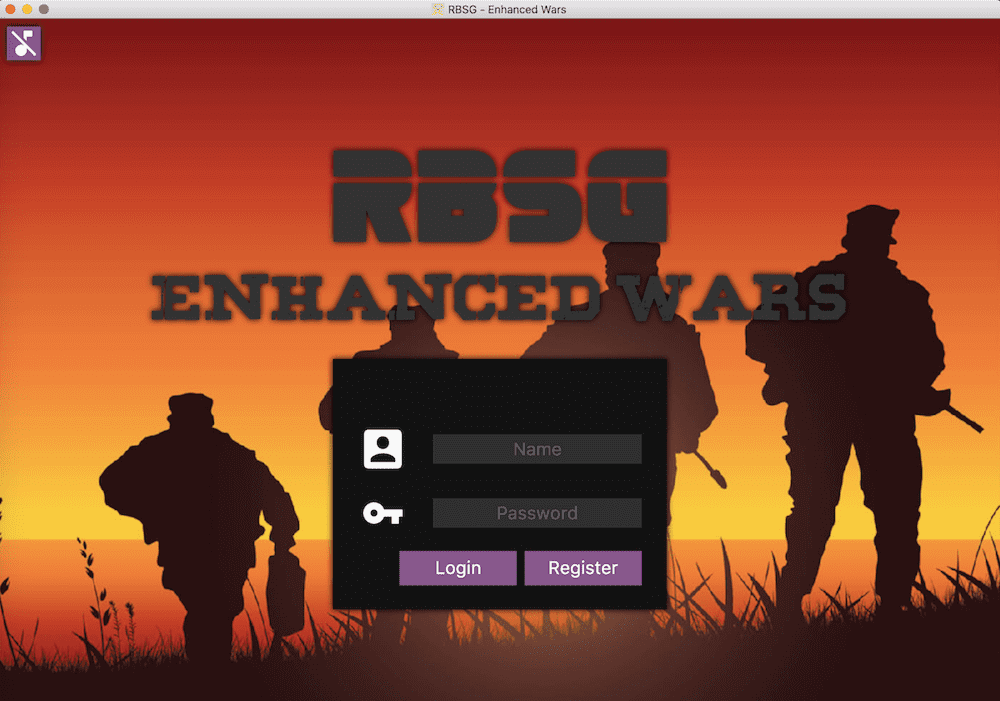
\includegraphics[width=0.8\textwidth]{images/old_state/login/Login.png}
    				\caption{Release \RN{2}: Login Szene}
    				\label{Login}
			    \end{figure}
			    \ \\ Versuchte der Nutzer sich anzumelden oder zu registrieren, erschien ein Lade-Indikator (siehe Abbildung \ref{Login_Form}) und die Buttons und Textfelder wurden disabled. Machte der Nutzer dabei einen Fehler oder konnte keine Verbindung zum Server hergestellt werden, erschien eine Fehlermeldung (siehe Abbildung \ref{Login_Form}). Der Login war internationalisiert und der Untertitel \glqq Enhanced Wars\grqq\ war animiert. Weiterhin konnte der Nutzer die Musik "uber den Musik Button in der Ecke ein- und ausschalten. \\
			    \begin{figure}[H]
                    \centering
                    \begin{subfigure}[h]{0.3\linewidth}
                        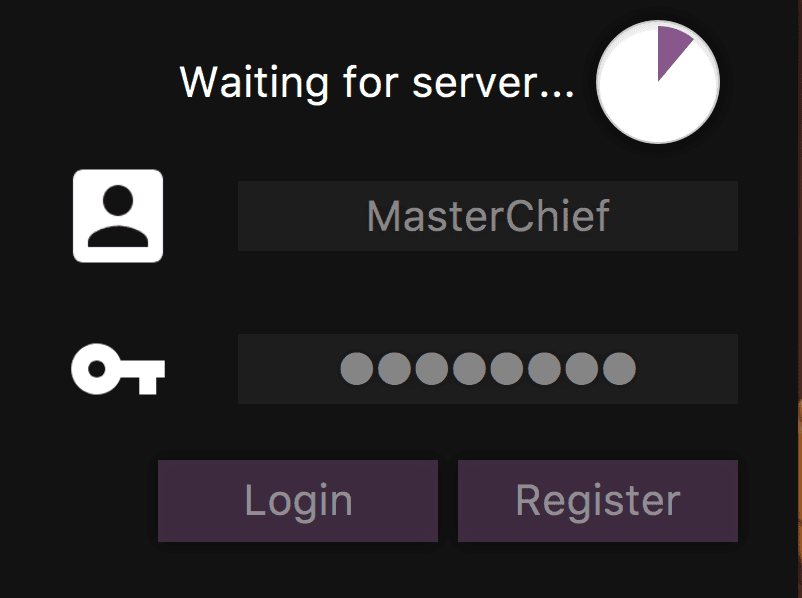
\includegraphics[width=\linewidth]{images/old_state/login/Indicator.png}
                        \caption{Indikator}
                    \end{subfigure}
                    \begin{subfigure}[h]{0.3\linewidth}
                        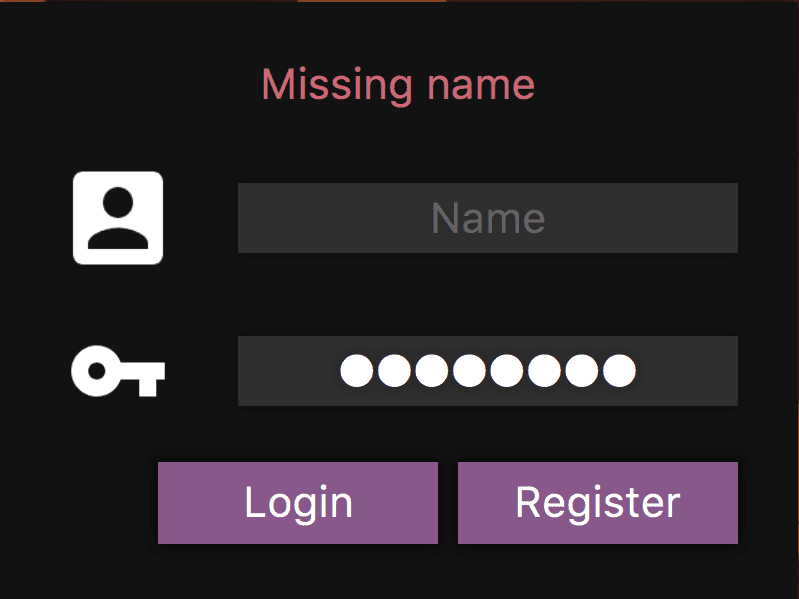
\includegraphics[width=\linewidth]{images/old_state/login/MissingName.png}
                        \caption{Missing Name}
                    \end{subfigure}
                    \begin{subfigure}[h]{0.3\linewidth}
                        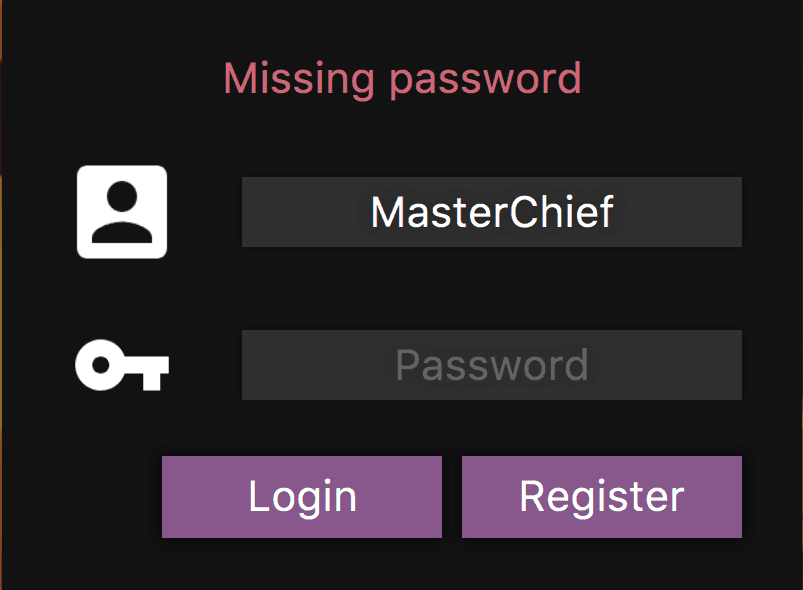
\includegraphics[width=\linewidth]{images/old_state/login/MissingPassword.png}
                        \caption{Missing Password}
                    \end{subfigure}
                    \begin{subfigure}[h]{0.3\linewidth}
                        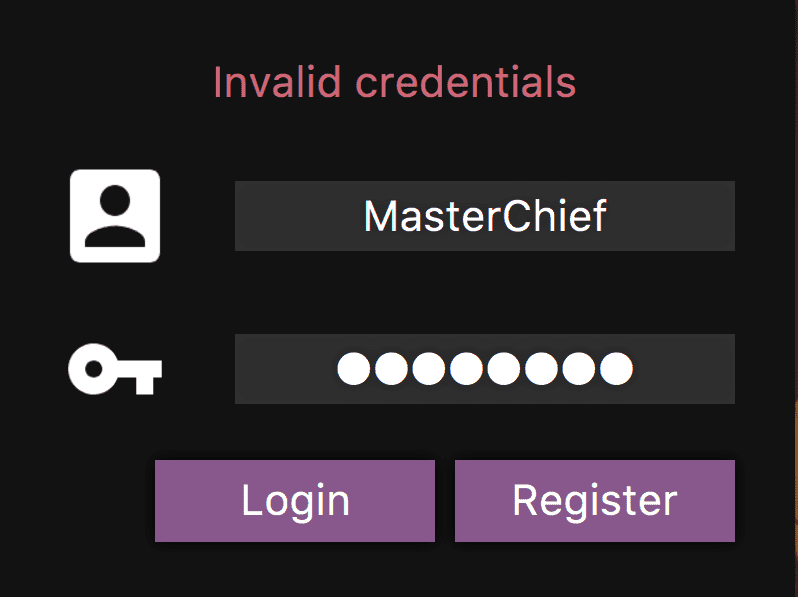
\includegraphics[width=\linewidth]{images/old_state/login/InvalidCredentials.png}
                        \caption{Invalid Credentials}
                    \end{subfigure}
                    \begin{subfigure}[h]{0.3\linewidth}
                        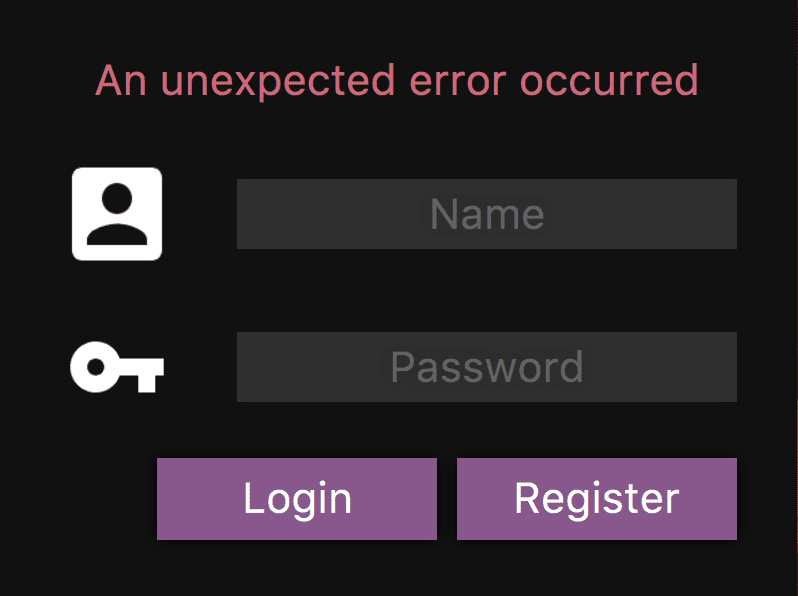
\includegraphics[width=\linewidth]{images/old_state/login/UnexpectedError.png}
                        \caption{Unexpected Error}
                    \end{subfigure}
                    \caption{Release \RN{2}: Login Formular}
                    \label{Login_Form}
                \end{figure}
            \subsubsection{Lobby} \label{LOBBY}
                Die Lobby zeigte eine Liste von allen Spielern (die nicht im Spiel waren) und allen Spielen an. Diese aktualisierten sich, wenn der Server die entsprechenede Nachricht schickte. Der Nutzer konnte sich "uber die Buttons oben rechts ausloggen, die Sprache "andern oder die Musik an- und ausschalten. Der Chat wurde unten links angezeigt. Rechts sah der Nutzer eine Liste mit allen vollst"andigen Armeen. Hatte der Nutzer keine vollst"andige Armee ausgew"ahlt, konnte er kein Spiel erstellen (siehe Abbildung \ref{Lobby_No_Army_Selected}) und auch keinem Spiel beitreten. \\
                \begin{figure}[H] 
    				\centering
    				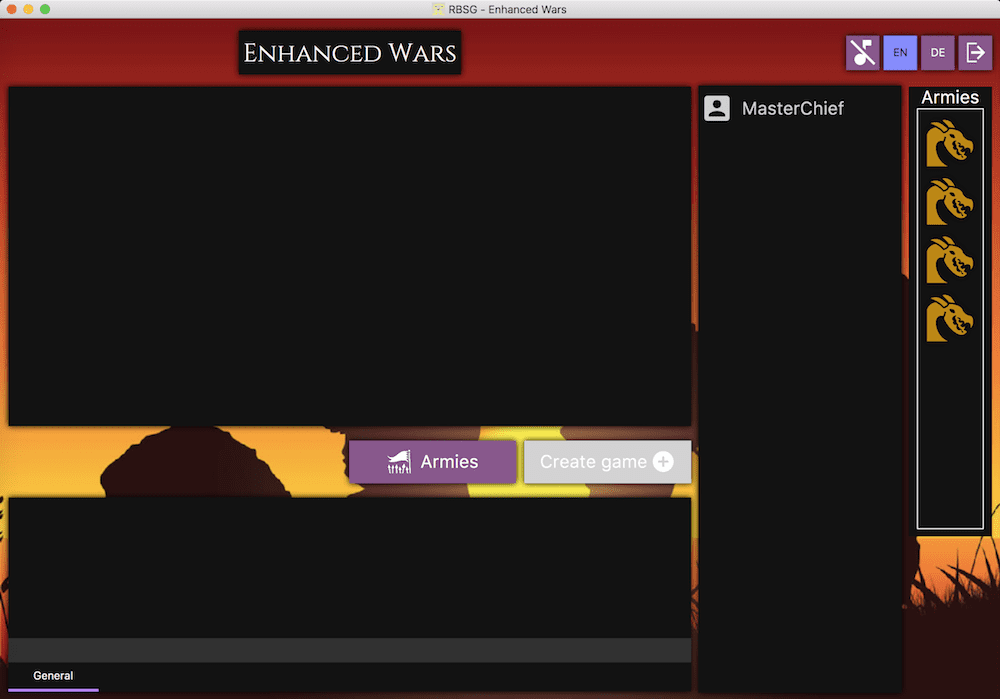
\includegraphics[width=0.8\textwidth]{images/old_state/lobby/NoArmySelected.png}
    				\caption{Release \RN{2}: Lobby Szene: Keine Armee ausgew"ahlt}
    				\label{Lobby_No_Army_Selected}
			    \end{figure}
			    \begin{wrapfigure}[8]{r}{0.35\textwidth}
                    \begin{center}
                        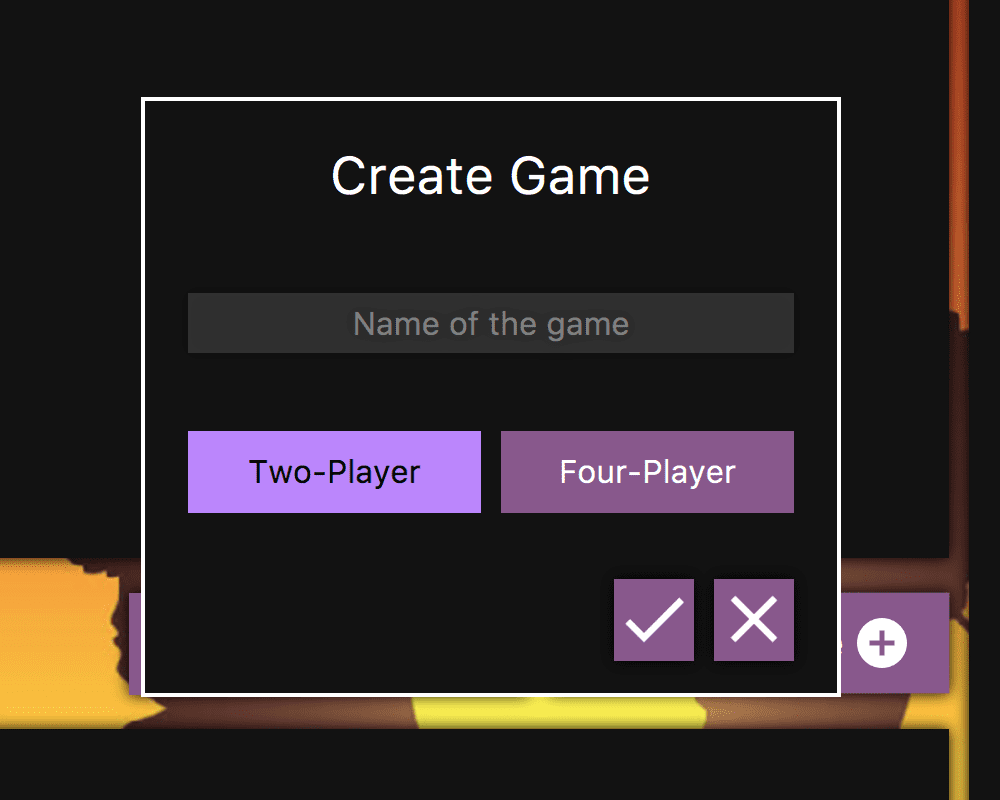
\includegraphics[width=0.35\textwidth]{images/old_state/lobby/CreateGame.png}
                    \end{center}
                    \caption{Release \RN{2}: Create Game Formular}
                    \label{Create_Game}
                \end{wrapfigure}
			    \ \vspace{0.5cm} \\ Hatte der Nutzer aber eine Armee ausgew"ahlt, konnte er ein Spiel erstellen oder einem Spiel beitreten (siehe Abbildung \ref{Create_Game} oder \ref{Lobby_Language}). Spiel erstellen funktionierte "uber den Create Game Button (siehe Abbildung \ref{Lobby_Army_Selected}). Der Nutzer hatte die Auswahl zwischen einem 2-Spieler-Spiel und einem 4-Spieler-Spiel. Danach wurde ein Autojoin gerufen und der Nutzer trat dem Spiel automatisch bei. Die Lobby war auch internationalisiert (vgl. Abbildung \ref{Lobby_Army_Selected} mit \ref{Lobby_Language}). \\
			    \begin{figure}[H] 
    				\centering
    				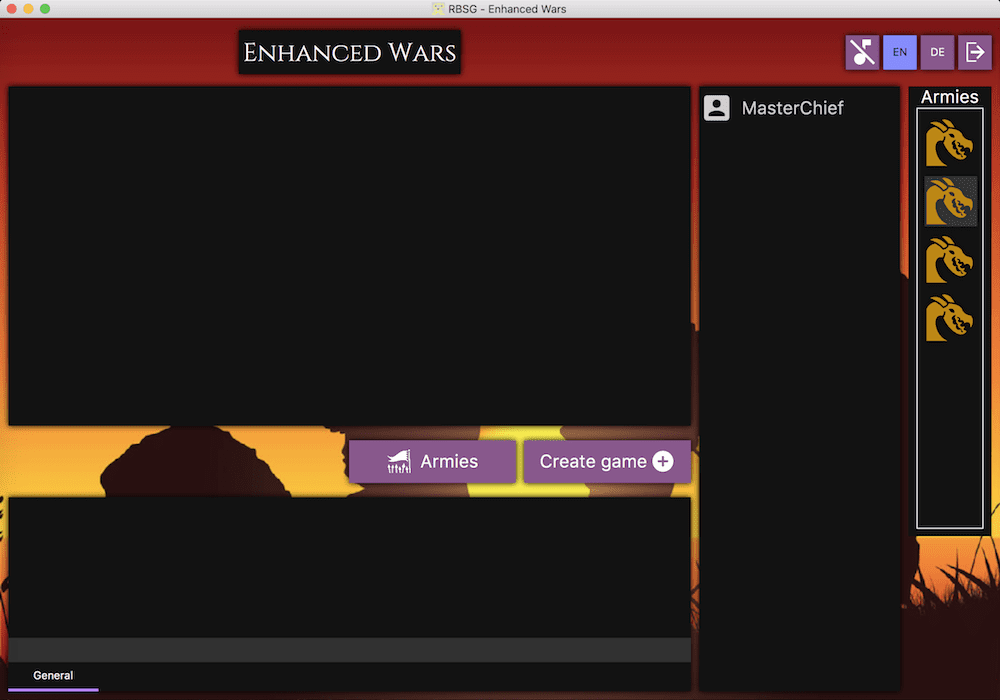
\includegraphics[width=0.8\textwidth]{images/old_state/lobby/ArmySelected.png}
    				\caption{Release \RN{2}: Lobby Szene: Armee ausgew"ahlt}
    				\label{Lobby_Army_Selected}
			    \end{figure}
			    \begin{figure}[H] 
    				\centering
    				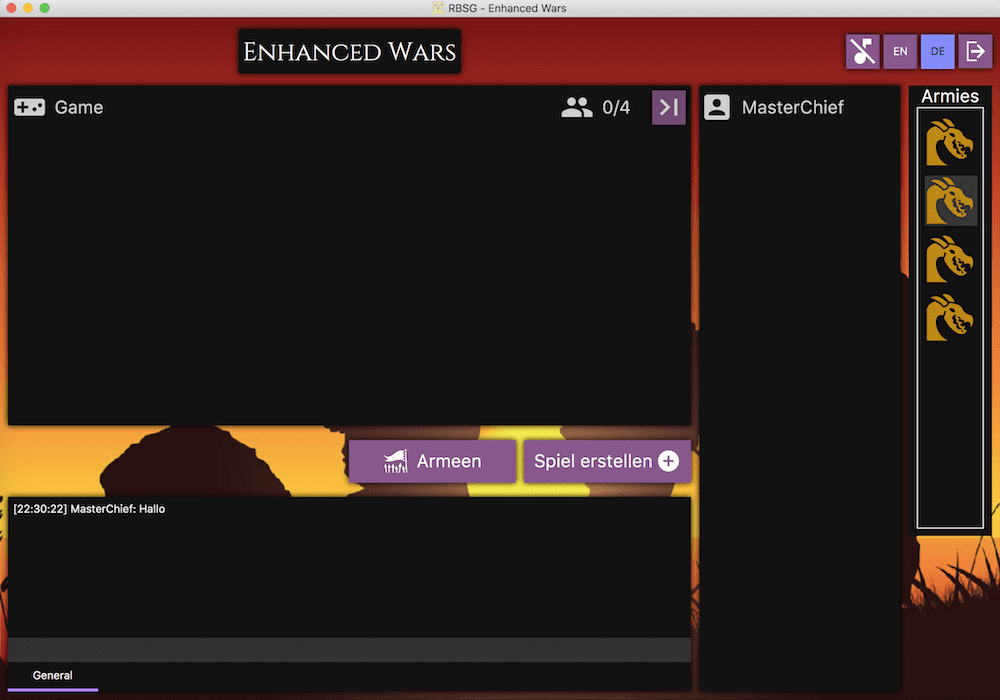
\includegraphics[width=0.8\textwidth]{images/old_state/lobby/International+Chat+GameCreated.png}
    				\caption{Release \RN{2}: Lobby Szene: Sprache DE}
    				\label{Lobby_Language}
			    \end{figure}
		    \subsubsection{Army Manager}
		        Im Army Manager gab es eine Liste der Einheiten, die der Nutzer w"ahlen konnte, und eine Liste der Einheiten, die in der gerade rechts ausgew"ahlten Armee waren. In der Mitte stand der Name der ausgew"ahlten Armee, ein Plus (+) und ein Minus (-) Button, um Einheiten der Armee hinzuzuf"ugen oder um sie zu l"oschen und ein Z"ahler, der anzeigte, wie viele Einheiten bereits in der Armee waren. Neben der Einheitenliste war eine Vorschau der gerade ausgew"ahlten Einheit. Neben diesem Feld wurden die Properties der Einheit angezeigt und welche Einheiten die ausgew"ahlte Einheit angreifen konnte. Hier stand bei keiner Auswahl in jedem Feld ein Fragezeichen (siehe Abbildung \ref{Army_Manager_No_Unit_Selected}), ansonsten Zahlenwerte (siehe Abbildung \ref{Army_Manager_Unit_Selected}). \\
		        \begin{figure}[H] 
    				\centering
    				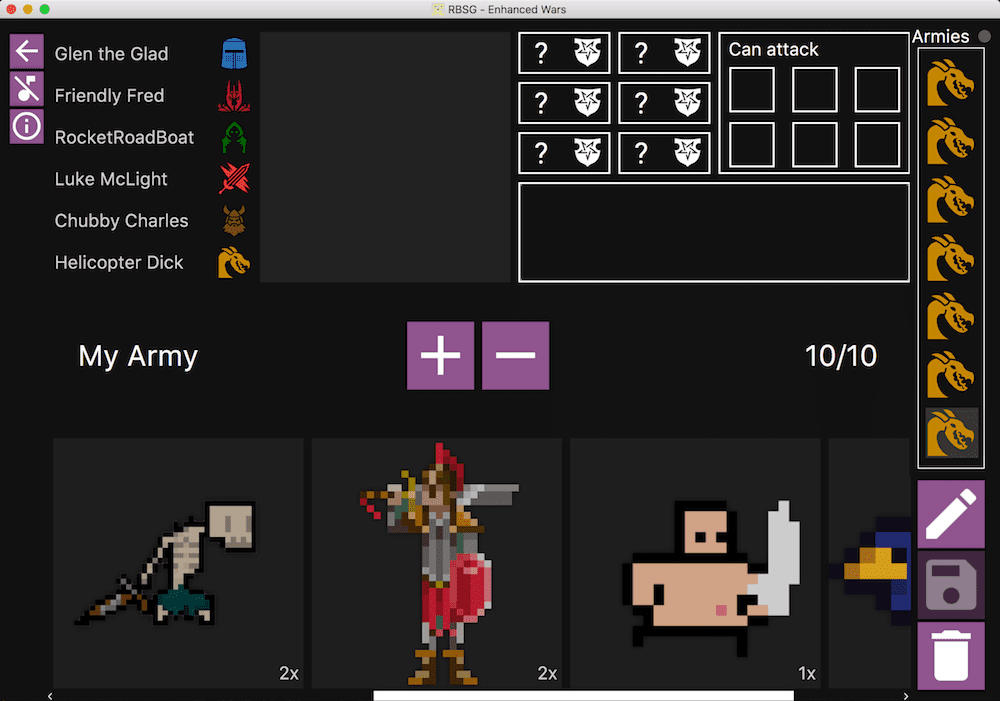
\includegraphics[width=0.8\textwidth]{images/old_state/army_manager/NoUnitSelected.png}
    				\caption{Release \RN{2}: Army Manager Szene: Keine Einheit ausgew"ahlt}
    				\label{Army_Manager_No_Unit_Selected}
			    \end{figure}
			    \begin{figure}[H] 
    				\centering
    				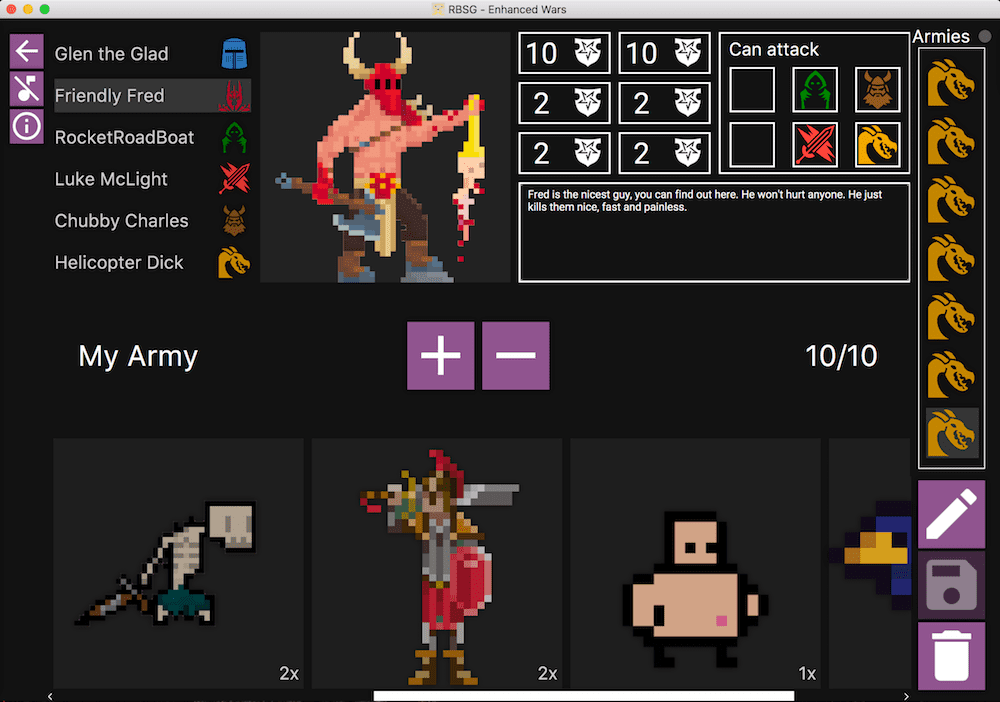
\includegraphics[width=0.8\textwidth]{images/old_state/army_manager/UnitSelected.png}
    				\caption{Release \RN{2}: Army Manager Szene: Einheit ausgew"ahlt}
    				\label{Army_Manager_Unit_Selected}
			    \end{figure}
			    \ \\ Darunter war der Lore Text der ausgew"ahlten Einheit zu sehen. Oben rechts waren Buttons, um zur"uck zur Lobby zu gehen, um die Musik ein- oder auszuschalten und ein Button, der die Properties in einem Overlay erkl"arte (siehe Abbildung \ref{Property_Infoo}). Unten rechts befanden sich Buttons, um eine Armee komplett zu l"oschen, \\
			    \begin{figure}[H]
                    \centering
                    \begin{minipage}{0.6\textwidth}
                        \centering
                        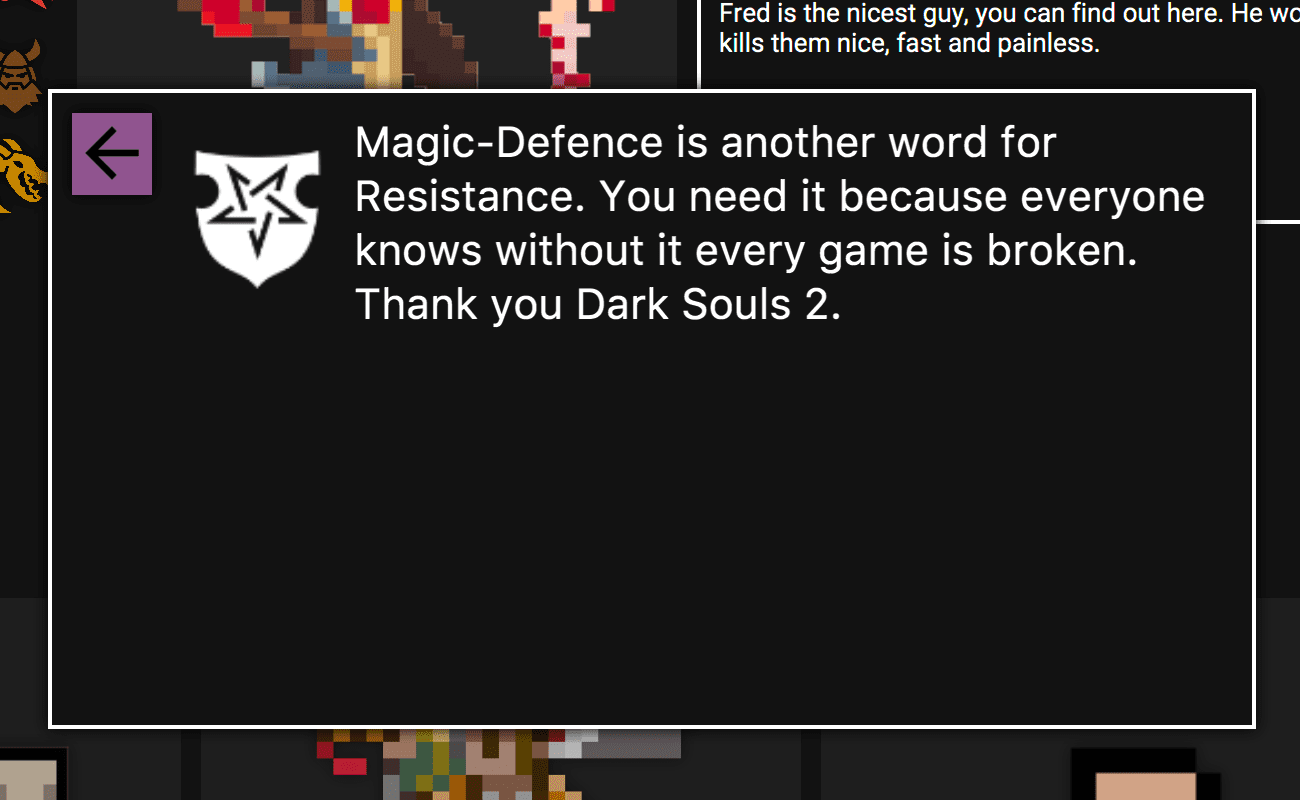
\includegraphics[width=0.6\textwidth]{images/old_state/army_manager/PropertyInfo.png}
                        \caption{Release \RN{2}: Property Info}
                        \label{Property_Infoo}
                    \end{minipage}%
                    \begin{minipage}{0.5\textwidth}
                        \centering
                        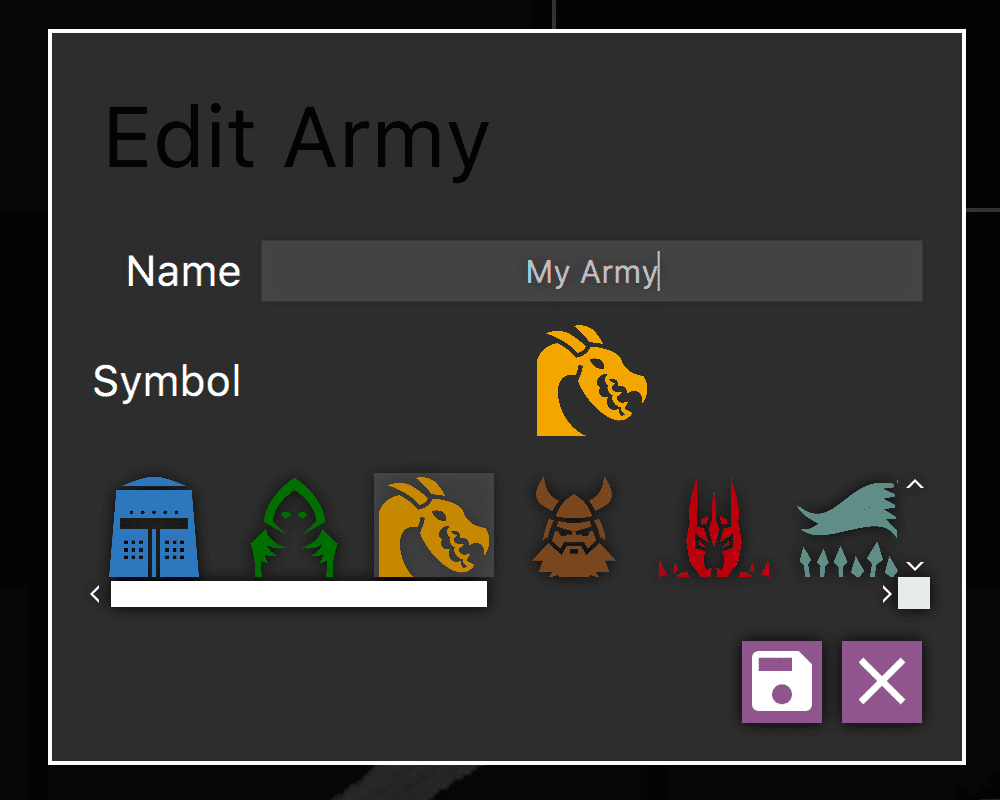
\includegraphics[width=0.5\textwidth]{images/old_state/army_manager/EditArmy.png}
                        \caption{Release \RN{2}: Armee bearbeiten}
                        \label{Edit_Army}
                    \end{minipage}
                \end{figure}
                \ \\ um sie zu speichern (wurde disabled, wenn sich nichts "anderte (siehe Abbildung \ref{Army_Manager_No_Unit_Selected}). Wenn der Nutzer aber etwas "anderte wurde der Button wieder enabled (siehe Abbildung \ref{Army_Manager_Ready_To_Save})). Es gab dort in der Ecke einen weiteren Button, um den Armeenamen zu "andern oder das Icon zu wechseln. Dazu "offnet sich ein weiteres Overlay (siehe Abbildung \ref{Edit_Army}). \\
                \begin{figure}[H] 
    				\centering
    				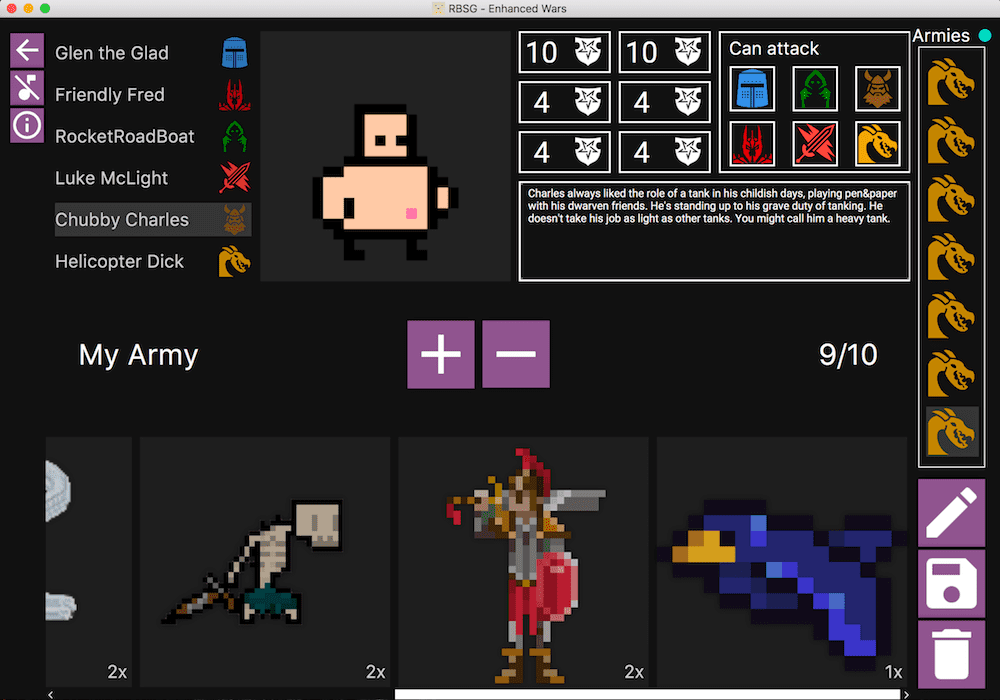
\includegraphics[width=0.8\textwidth]{images/old_state/army_manager/ArmyReadyToSave.png}
    				\caption{Release \RN{2}: Army Manager Szene: Speicherbar}
    				\label{Army_Manager_Ready_To_Save}
			    \end{figure}
	        \subsubsection{Waiting Room (Gamelobby)} \label{WAITING_ROOM}
                Trat der Nutzer dem Warteraum bei, dann sah er oben rechts verschiedene Buttons. Einmal einen Button zum Verlassen des Spiels in die Lobby, einen Button, um die Musik ein- und auszuschalten, und einen Button, um Informationen anzuzeigen. Da dieser Button noch keine spezielle Funktion hatte, wechselte der Nutzer mit diesem testweise auf das Spielfeld (Ingame). Oben in der Mitte wurde die Kartenvorschau angezeigt. \\
                \begin{figure}[H] 
    				\centering
    				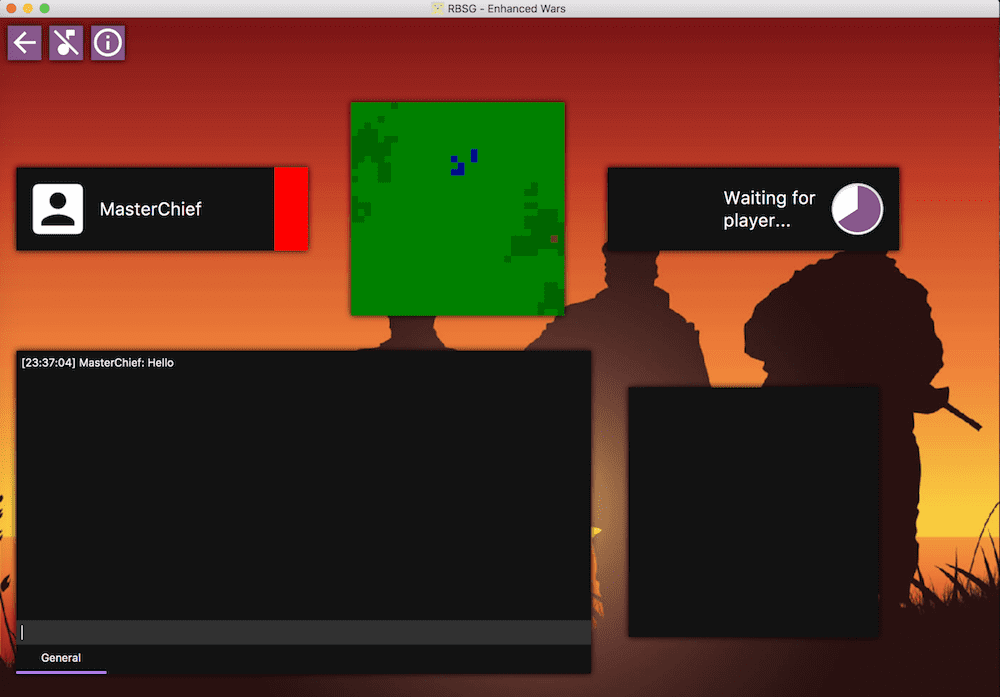
\includegraphics[width=0.8\textwidth]{images/old_state/waiting_room/2Player.png}
    				\caption{Release \RN{2}: Waiting Room Szene: 2 Spieler}
    				\label{Waiting_Room_2}
			    \end{figure}
			    \begin{figure}[H] 
    				\centering
    				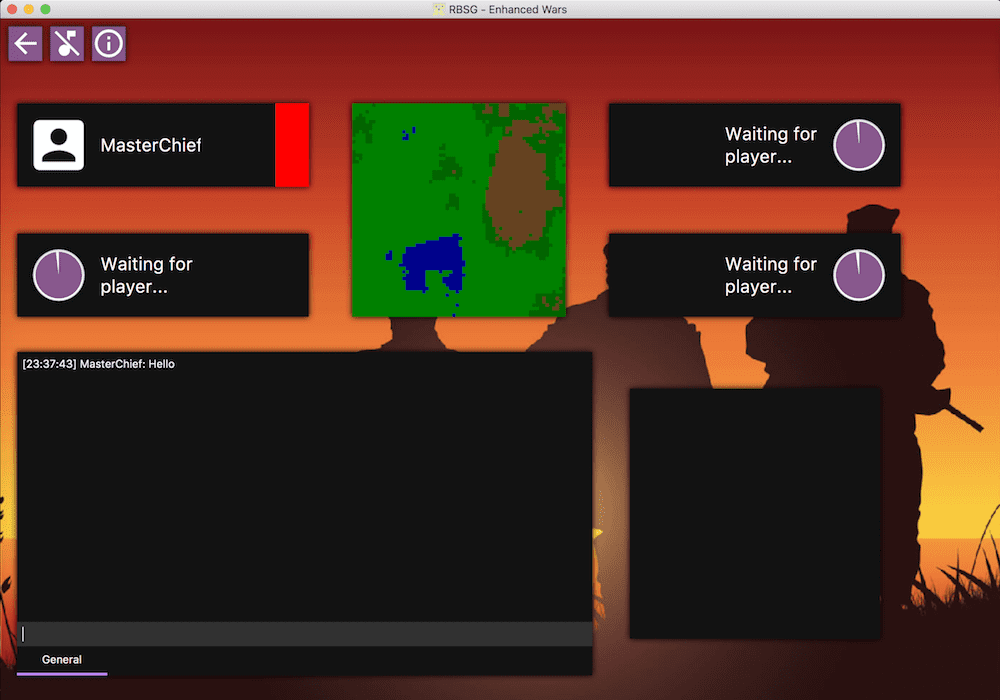
\includegraphics[width=0.8\textwidth]{images/old_state/waiting_room/4Player.png}
    				\caption{Release \RN{2}: Waiting Room Szene: 4 Spieler}
    				\label{Waiting_Room_4}
			    \end{figure}
			    \ \\ Links und rechts daneben waren die Spielerkarten zu sehen. Je nachdem ob der Nutzer ein 2-Spieler-Spiel oder ein 4-Spieler-Spiel startete, befanden sich dort zwei oder vier Spielerkarten (siehe Abbildung \ref{Waiting_Room_2} und \ref{Waiting_Room_4}). Auf den Spielerkarten fanden sich der Name und die Farbe des jeweiligen Spielers vor. Waren noch nicht genug Spieler dem Spiel beigetreten, wurden Lade-Indikatoren in den Spielerkarten angezeigt. Unten war der Chat und daneben eine freie Pane f"ur ein Minigame, dass noch implementiert werden sollte.
	        \subsubsection{Ingame}
	            Die Ingameszene zeigte bisher nur die Karte und das initiale Spielgeschehen. Die initialen Einheiten wurden auch angezeigt. Weiterhin gab es einen Button, der zur"uck in die Lobby navigierte. Zwei weitere Buttons kontrollierten das Zoomen auf dem Spielfeld (siehe Abbildung \ref{Ingame}, \ref{Ingame_In} und \ref{Ingame_Out}). \\
	            \begin{figure}[H] 
    				\centering
    				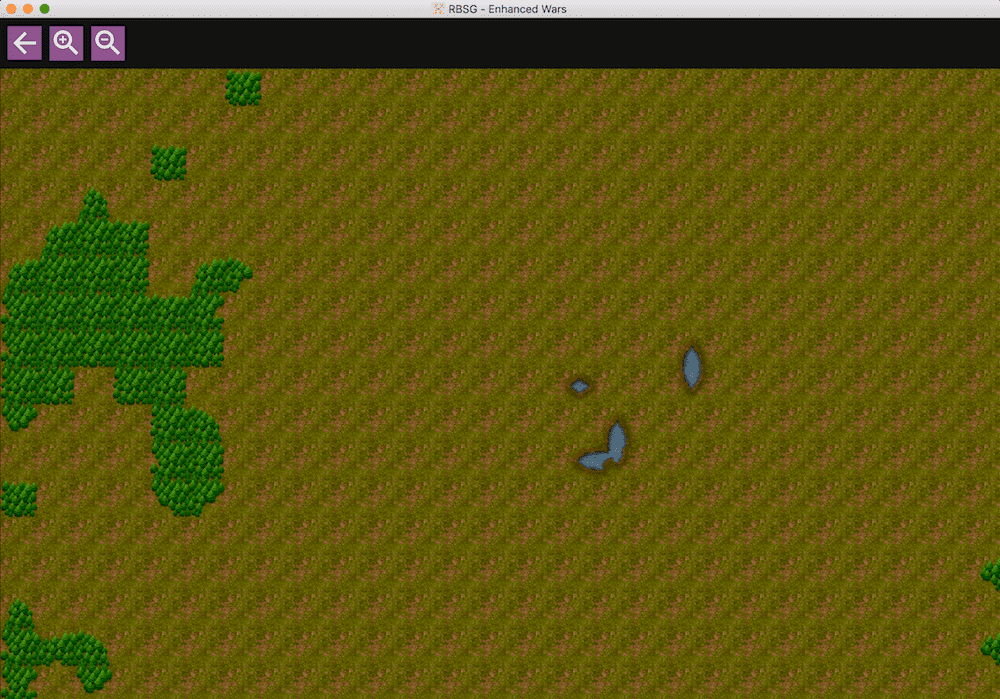
\includegraphics[width=0.8\textwidth]{images/old_state/ingame/Ingame.png}
    				\caption{Release \RN{2}: Ingame Szene}
    				\label{Ingame}
			    \end{figure}
			    \begin{figure}[H] 
    				\centering
    				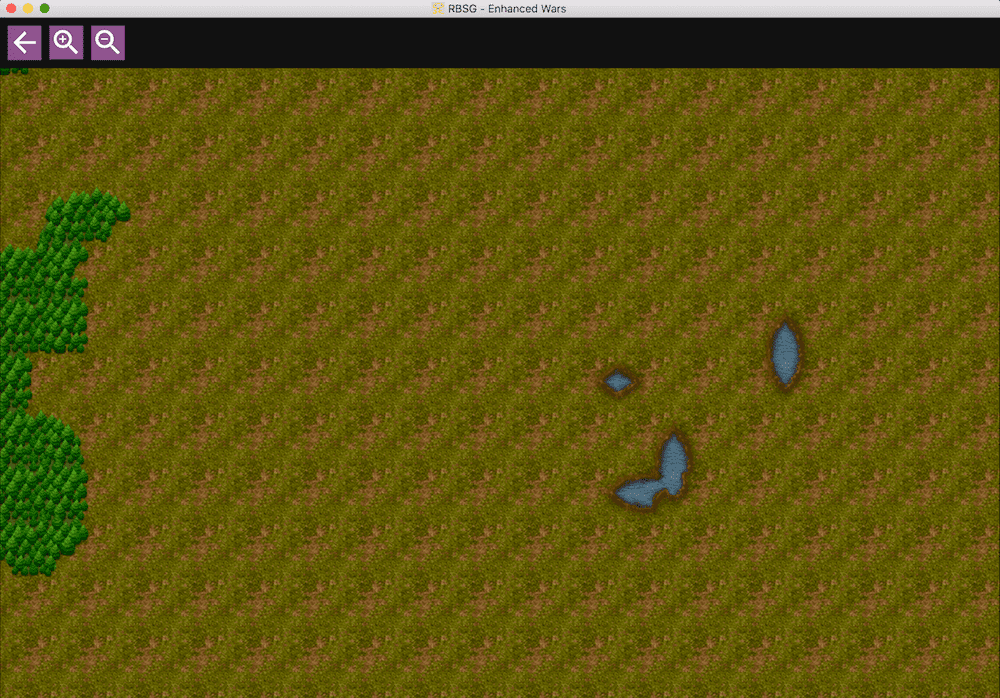
\includegraphics[width=0.8\textwidth]{images/old_state/ingame/ZoomIn.png}
    				\caption{Release \RN{2}: Ingame Szene: Zoom In}
    				\label{Ingame_In}
			    \end{figure}
			    \begin{figure}[H] 
    				\centering
    				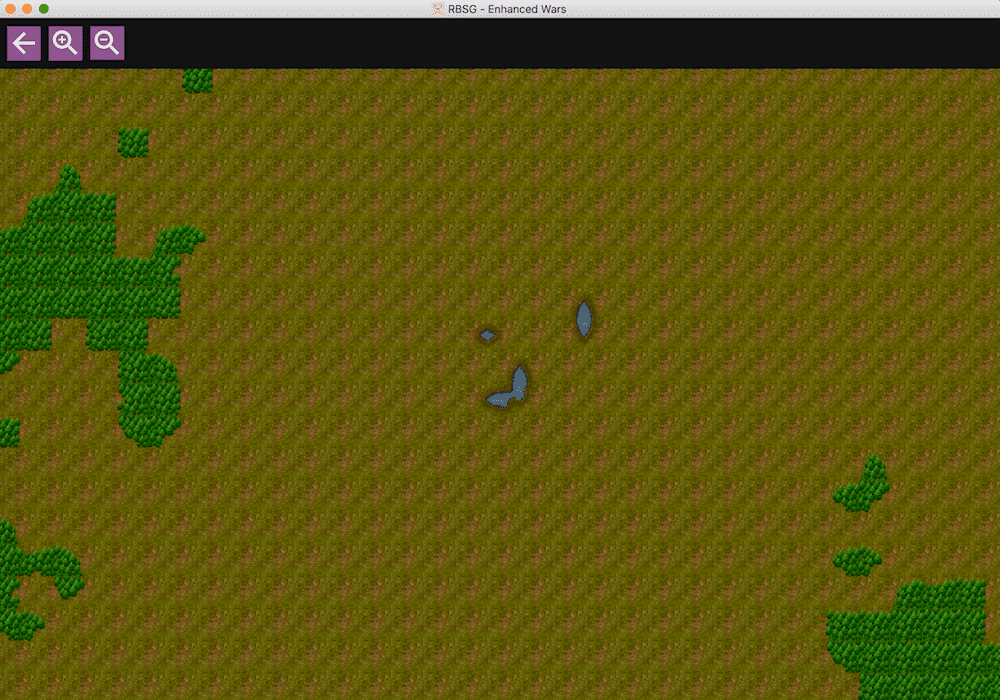
\includegraphics[width=0.8\textwidth]{images/old_state/ingame/ZoomOut.png}
    				\caption{Release \RN{2}: Ingame Szene: Zoom Out}
    				\label{Ingame_Out}
			    \end{figure}
	\newpage
		    \subsubsection{Weitere Features}
		        \begin{wrapfigure}[23]{r}{0.35\textwidth}
                    \begin{center}
                        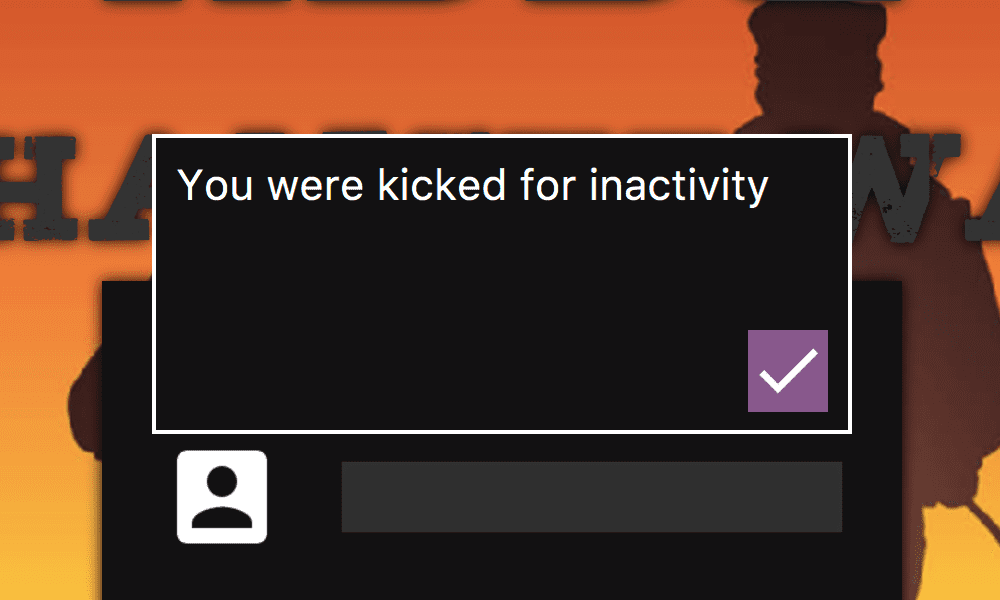
\includegraphics[width=0.35\textwidth]{images/old_state/additional/LoginFailure.png}
                        \caption{Release \RN{2}: Login Fehler}
                        \label{Login_Failure}
                    \end{center}
                    \begin{center}
                        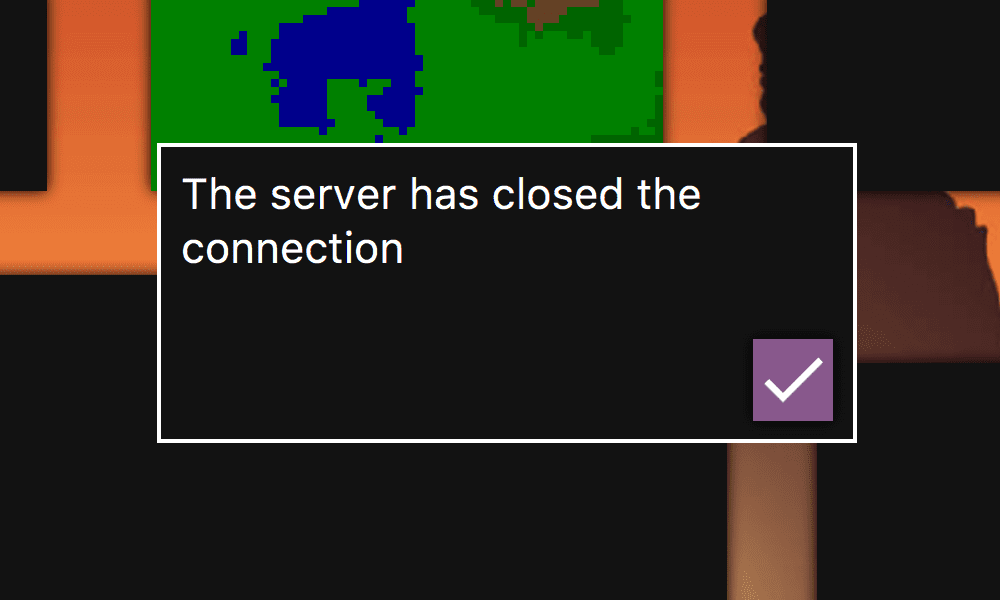
\includegraphics[width=0.35\textwidth]{images/old_state/additional/WaitingRoomFailure.png}
                        \caption{Release \RN{2}: Spielfehler}
                        \label{Game_Failure}
                    \end{center}
                \end{wrapfigure}
		        \ \\ Weiterhin wurde seit den ersten beiden Releases ein Dark Theme Styling implementiert, wie auf allen vorangegangenen Abbildungen zu sehen ist. Musik und Internationalisierung waren zwar optional, aber funktionierten in jeder Szene. Der Nutzer konnte auch nach Belieben Chuck Norris Zitate "uber den Chat-Befehl \glqq \textbackslash chuckMe\grqq\ im Chat versenden und es wurde auch mit einem Zeitstempel vor jeder Nachricht angezeigt, wann sie verschickt wurde. Wenn der Nutzer eine private Nachricht bekam, wurde dies auf dem neu aufgegangenem Tab mit der secondary Farbe signalisiert. Die Kartenvorschau im Warteraum war auch optional, genauso wie das Zoomen Ingame. Den Armeenamen, sowie das Icon dazu "andern zu k"onnen, war auch optional. Der Autojoin nach dem Create Game wurde auch nicht verlangt, funktioniert aber bestens. Ein weiteres sehr wichtiges Feature war, dass der Client den Spieler Fehlermeldungen (siehe Abbildung \ref{Login_Failure} und \ref{Game_Failure}) schickte, wenn der Server einen Websocket unerwartet schlo"ss. Der Nutzer wurde je nach Fehler in den Login oder die Lobby zur"uckgeschickt. Au"sserdem gab es ein Fenster, in dem sich der Nutzer noch einmal entscheiden konnte, ob er sich wirklich ausloggen oder ob er wirklich das Spiel verlassen mochte (siehe Abbildung \ref{Leave_Game} und \ref{Logout}). \\
		        \begin{figure}[H]
                    \centering
                    \begin{minipage}{0.55\textwidth}
                        \centering
                        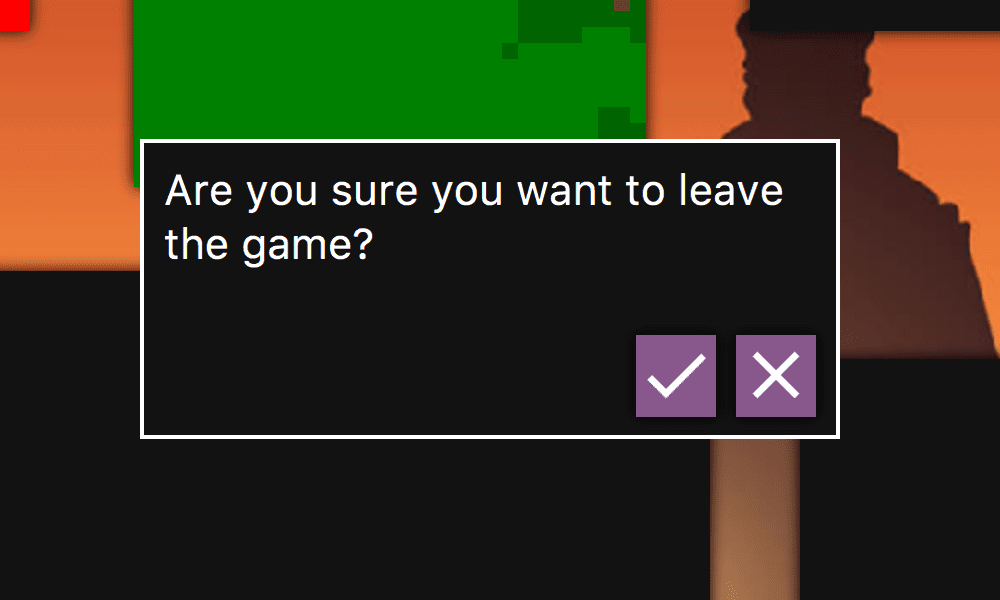
\includegraphics[width=0.55\textwidth]{images/old_state/additional/LeaveGame.png}
                        \caption{Release \RN{2}: Spiel verlassen}
                        \label{Leave_Game}
                    \end{minipage}%
                    \begin{minipage}{0.55\textwidth}
                        \centering
                        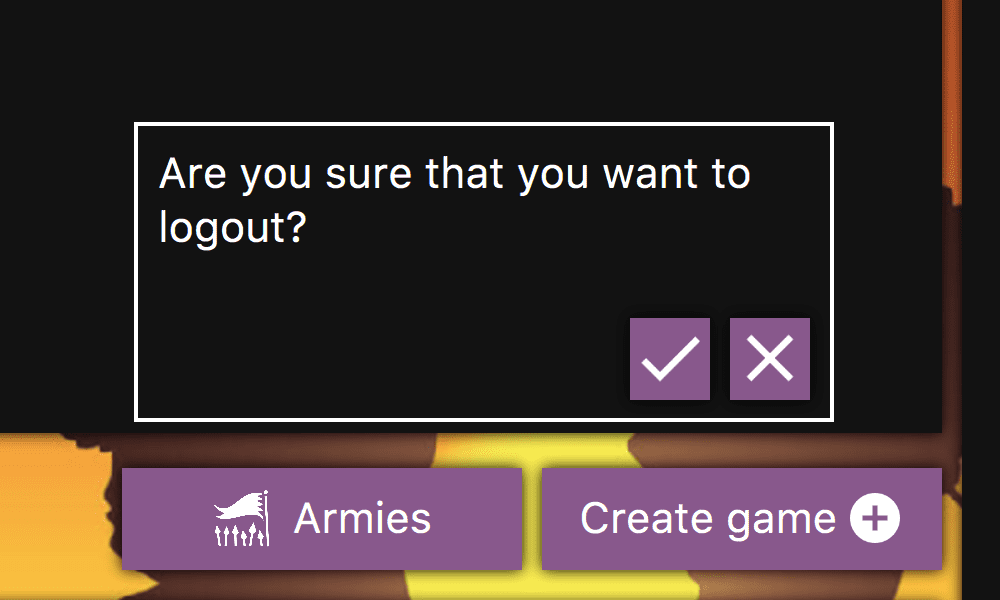
\includegraphics[width=0.55\textwidth]{images/old_state/additional/Logout.png}
                        \caption{Release \RN{2}: Logout}
                        \label{Logout}
                    \end{minipage}
                \end{figure}
                \ \\ Die C0 Testabdeckung betrug zum Ende des Releases \RN{2} 77\%.
                \begin{figure}[H] 
    				\centering
    				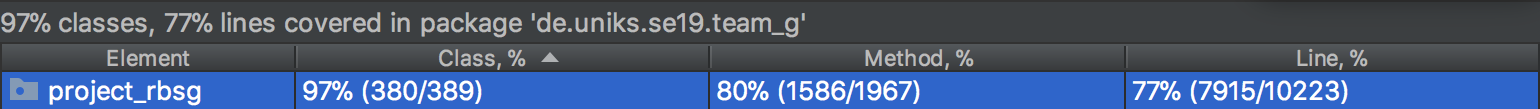
\includegraphics[width=0.8\textwidth]{images/old_state/Coverage.png}
    				\caption{Release \RN{2}: C0 Testabdeckung (Siehe Line, \%)}
    				\label{Coverage}
			    \end{figure}
    \newpage
	    \subsection{MockUps}
	        Aufgrund der Releaseanforderungen wurden f"ur das Kundentreffen am 1.7.2019 MockUps zu der neuen Ingame Szene erstellt. Weiterhin gab es auch noch MockUps zur Lobby und zum Waiting Room. Diese wurden nach dem Erscheinen der Serverdokumentation noch erweitert. Im sechsten Sprint wurden die MockUps auch noch einmal angepasst, da sich grundlegende \"Anderungen ergeben haben (Ein Kontextmen"u wurde durch eine Sidebar ersetzt. Die MockUps waren im Stil des Dark Theme und sollten an die UI aus den vorherigen Releases ankn"upfen.
	        \subsubsection{Lobby}
	           Es wurde gefordert, in der Lobby ein Button hinzuzuf"ugen, der es dem Nutzer erlaubt einem Beobachtungsmodus beizutreten. Des Weiteren sollte die Armeeauswahl aus der Lobby entfernt werden (und in den Waiting Room verlegt werden). \\
	            \begin{figure}[H] 
    				\centering
    				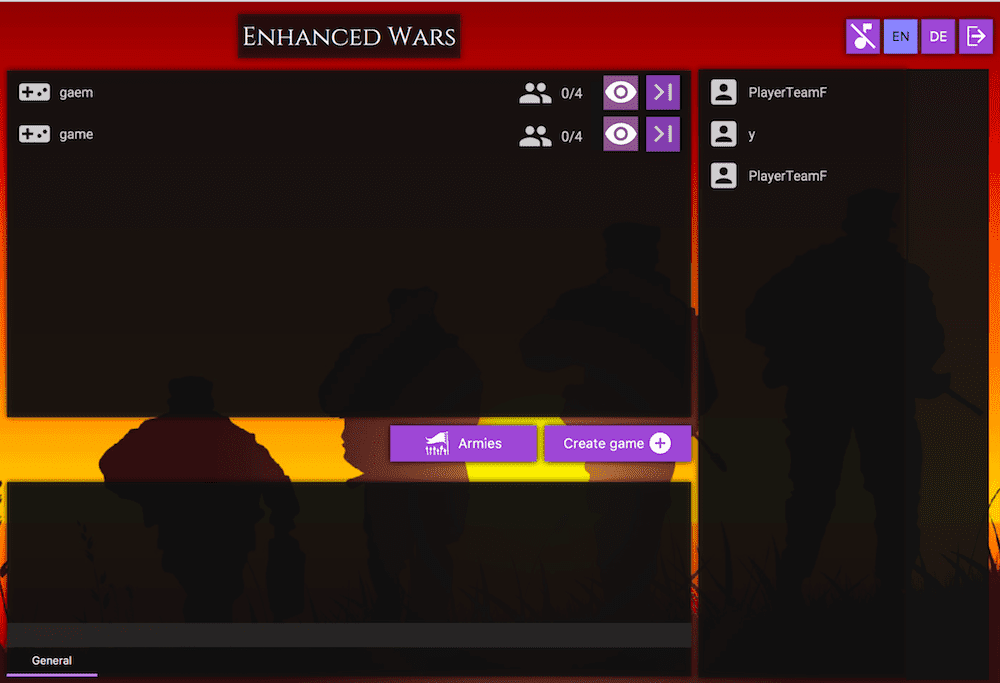
\includegraphics[width=0.8\textwidth]{images/mockUps/LobbyWatchMode.png}
    				\caption{MockUp: Beobachtungsmodus Lobby}
    				\label{Watch_Mode}
			    \end{figure}
		    \subsubsection{Waiting Room (Gamelobby)}
		        Da der Waiting Room im Release \RN{2} (siehe Kapitel \ref{WAITING_ROOM}) schon gr"o"sstenteils vorhanden war, musste nur noch das Ready geben hinzugef"ugt werden. Dies sollte bei uns passieren, wenn man eine Armee ausw"ahlt (siehe Abbildung \ref{Ready}). Die Armeeauswahl musste deswegen von der Lobby in den Waiting Room umgezogen werden. Spieler, die bereits bereit waren, sollten in ihrer Playercard in der secondary Farbe hinterlegt werden und die Icons sollten sich schwarz f"arben. Wenn alle Spieler das Ready gaben, wurde ein Overlay angezeigt, in dem ein Indikator lud, bis zur Ingame Szene gewechselt wurde (siehe Abbildung \ref{Game_Start}). Auf den MockUps waren auch zwei optionale Features zu sehen. Dies war einmal das TicTacToe Spiel unten rechts, das gegebenenfalls implementiert werden sollte. Und au"sserdem sollte oben in der Mitte der Name des Spiels angezeigt werden (siehe auf den MockUps mit Beispielnamen \glqq Enhanced Wars\grqq). \\
		        \begin{figure}[H] 
    				\centering
    				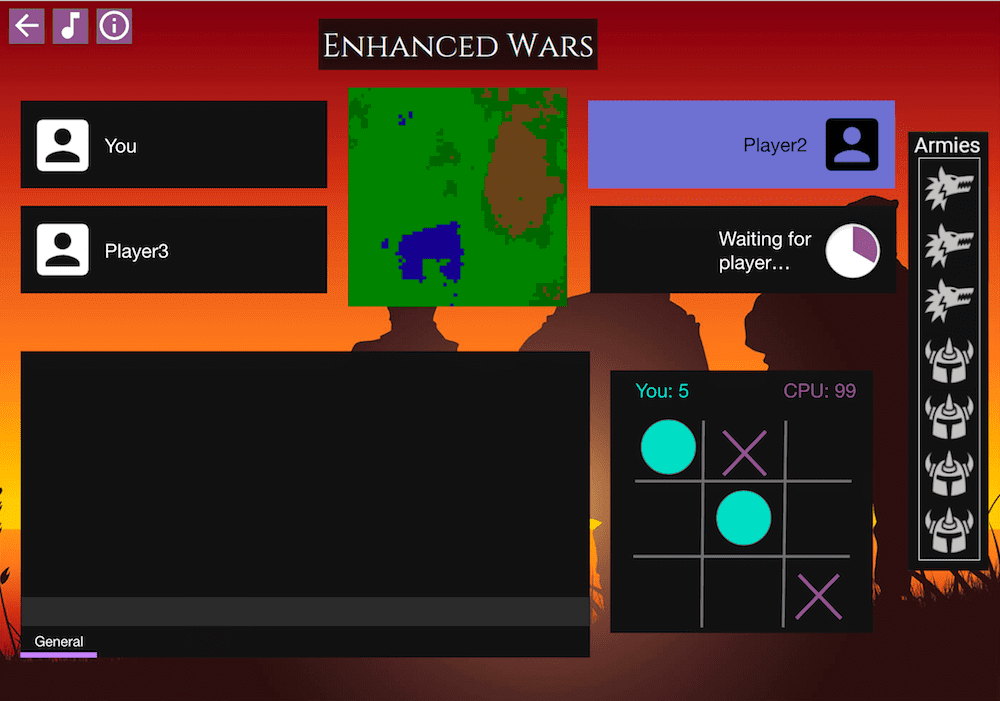
\includegraphics[width=0.8\textwidth]{images/mockUps/NotReady.png}
    				\caption{MockUp: Nutzer nicht bereit}
    				\label{Not_Ready}
			    \end{figure}
			    \begin{figure}[H] 
    				\centering
    				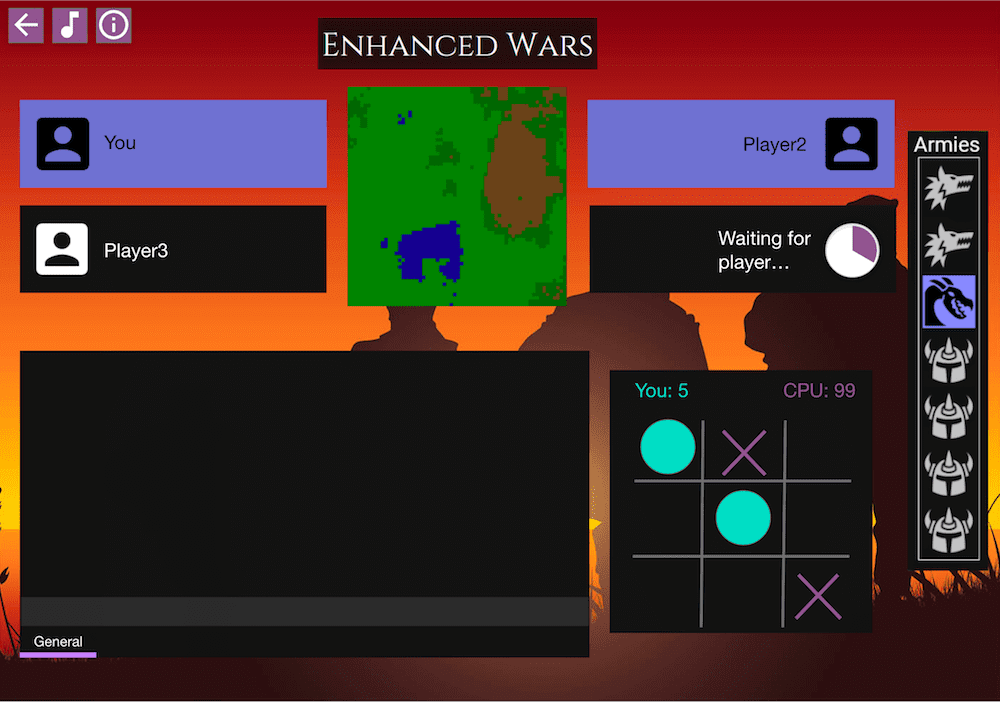
\includegraphics[width=0.8\textwidth]{images/mockUps/Ready.png}
    				\caption{MockUp: Nutzer bereit}
    				\label{Ready}
			    \end{figure}
			    \begin{figure}[H] 
    				\centering
    				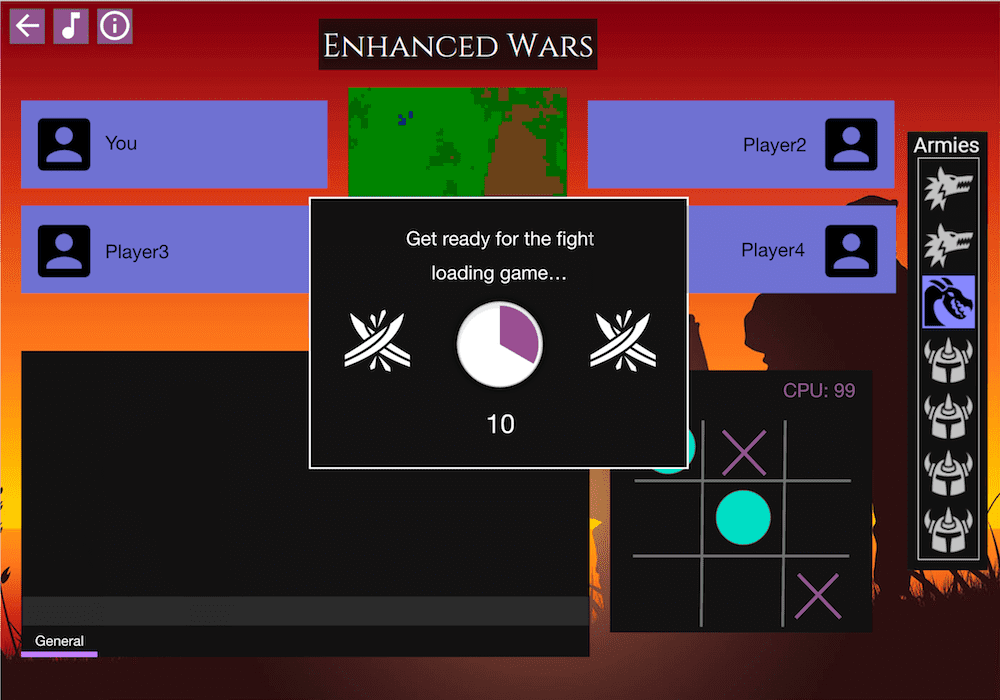
\includegraphics[width=0.8\textwidth]{images/mockUps/StartGame.png}
    				\caption{MockUp: Spielstart}
    				\label{Game_Start}
			    \end{figure}
		    \subsubsection{Ingame}
		        Bisher zeigte die Ingame Szene nur das initiale Spielgeschehen. In diesem Release sollte diese Szene haupts"achlich erweitert werden. Chat, die Minikarte und die Spieler mussten angezeigt werden. \\
		        \begin{figure}[H] 
    				\centering
    				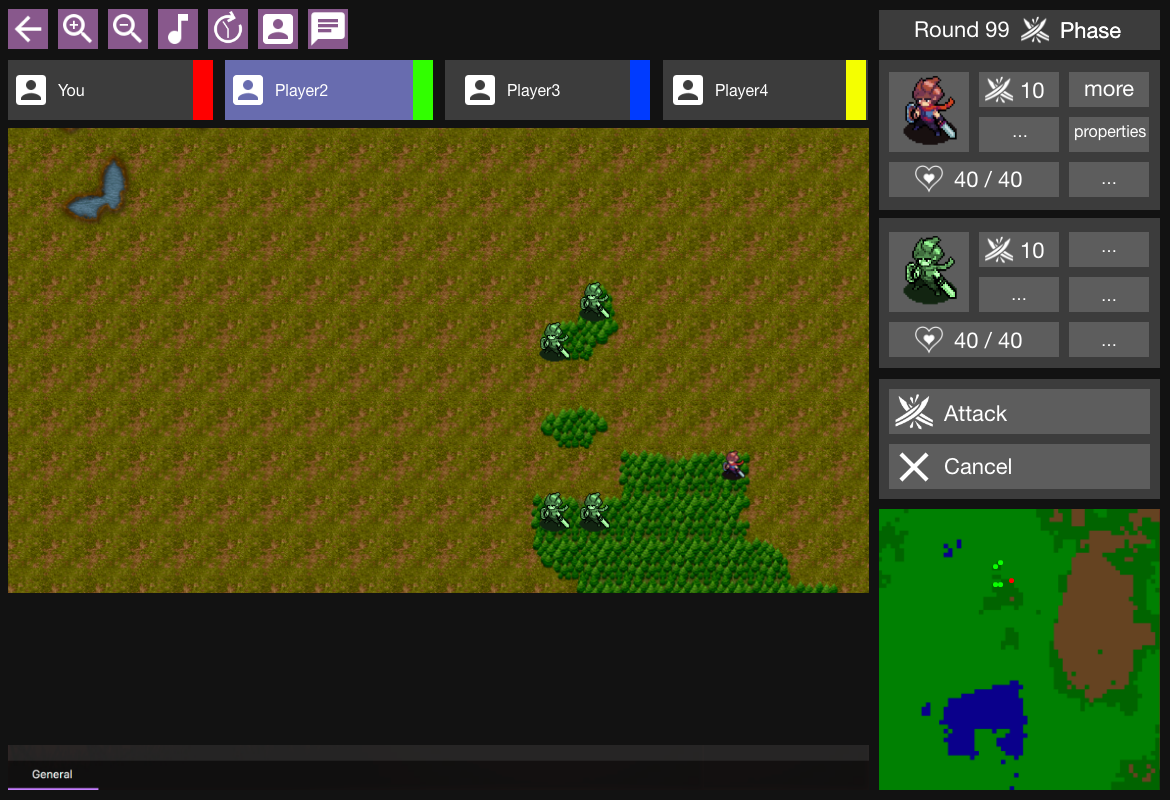
\includegraphics[width=0.8\textwidth]{images/mockUps/Ingame.png}
    				\caption{MockUp: Ingame}
    				\label{Ingame_View}
			    \end{figure}
		    	\ \\   Der Chat und die Spielerkarten sollten auch "uber die jeweiligen Buttons oben in der Leiste eingeklappt werden k"onnen und Overlays "uber dem Spielfeld sein. Die Minikarte sollte unten rechts unter der Sidebar angezeigt werden. Die Sidebar war eine neue feste Box rechts neben dem Spielfeld. Diese sollte die Einheiteninformationen und die Best"atigen/Abbrechen Buttons enthalten. Die aktuelle Runde und die aktuelle Phase sollten oben "uber der Sidebar angezeigt werden. Der aktuelle Spieler sollte in seiner Playercard mit der secondary Farbe hinterlegt werden. In der oberen Leiste kam au"sserdem der Musik Button zum ein- und ausschalten der Musik hinzu.
			    \subsubsubsection{Einheit ausw"ahlen}
			        Der Server stellte drei Phasen zur Verf"ugung, wenn ein Spieler an der Reihe war. Eine Bewegungsphase, in der mindestens eine Einheit bewegt werden musste, eine Angriffsphase, die "ubersprungen werden konnte und eine restliche Bewegungspunktephase, die ebenfalls "ubersprungen werden konnte. \\
			        \begin{figure}[H] 
    				    \centering
    				    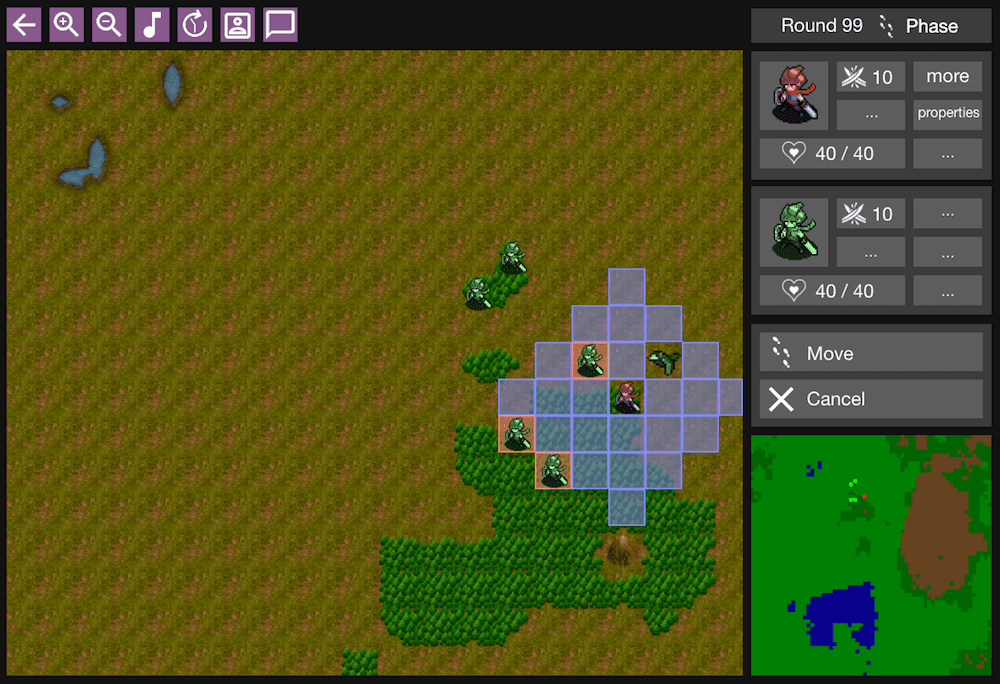
\includegraphics[width=0.8\textwidth]{images/mockUps/Select.png}
    				    \caption{MockUp: Phase 1: Ausw"ahlen}
    				    \label{Select_1}
			        \end{figure}
			        \ \\ Nachdem alle drei Phasen vom aktiven Spieler beendet wurden, war die Runde des Spielers vorbei. Wenn der Nutzer selbst an der Reihe war und in einer seiner drei Phasen auf eine Einheit klickte, sollte der Bewegungsradius oder Angriffsradius angezeigt werden. Klickte der Nutzer wieder auf die bereits ausgew"ahlte Einheit, auf eine andere Einheit oder auf ein freies Feld, dann sollte die Einheit nicht mehr ausgew"ahlt sein. \\
                    \begin{figure}[H] 
    				    \centering
    				    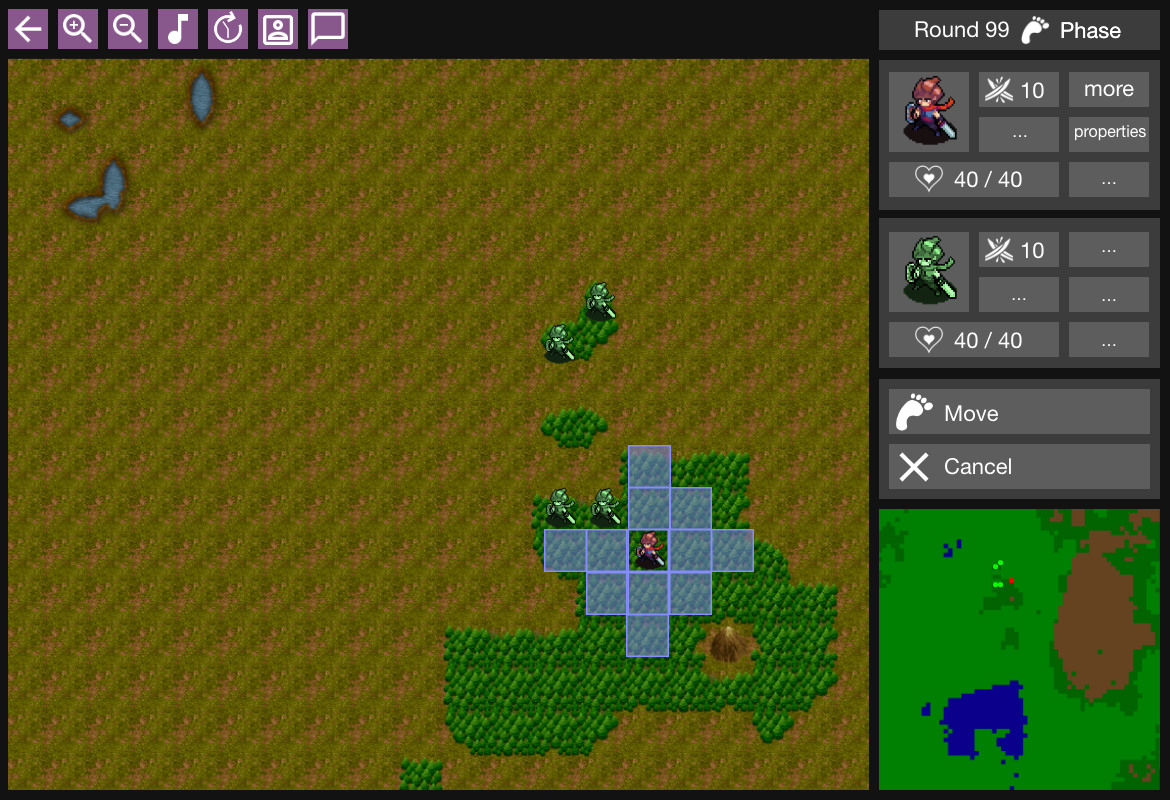
\includegraphics[width=0.8\textwidth]{images/mockUps/Select2.png}
    				    \caption{MockUp: Phase 2: Ausw"ahlen}
    				    \label{Select_2}
			        \end{figure} 
			        \begin{figure}[H] 
    				    \centering
    				    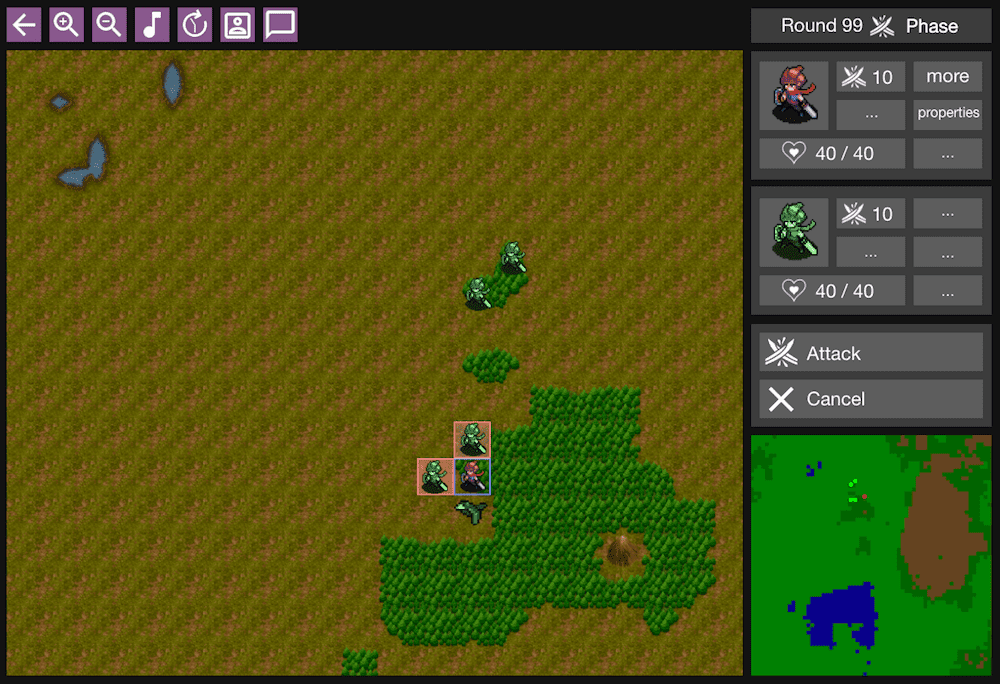
\includegraphics[width=0.8\textwidth]{images/mockUps/Select3.png}
    				    \caption{MockUp: Phase 3: Ausw"ahlen}
    				    \label{Select_3}
			        \end{figure} 
		            \ \\ In einer gegnerischen Phase sollte die Einheit, die vom Gegner in seinem Client ausgew"ahlt wurde, auch beim Nutzer, w�hrenddessen der Nutzer dem Gegner zuschaute, auf die selbe Art und Weise ausgew"ahlt werden. In Phase 1 sollten zus"atzlich zum Bewegungsradius auch alle m"oglichen Angriffsziele markiert werden (siehe Abbildung \ref{Select_1}). In Phase 2 sollten nur alle m"oglichen Angriffsziele angezeigt werden (siehe Abbildung \ref{Select_2}). In Phase 3 sollte ein verk"urzter Bewegungsradius ohne Angriffsziele angezeigt werden (siehe Abbildung \ref{Select_3}), je nachdem wie weit sich eine Einheit noch bewegen konnte.
                \subsubsubsection{Einheit bewegen}
                    Nachdem der Nutzer in Phase 1 oder 3 eine Einheit ausgew"ahlte und auf ein Feld klickte, sollte die Einheit auf das Feld bewegt werden, sobald der k"urzeste Pfad berechnet und zum Server geschickt wurde. Falls nach der Bewegung noch Bewegungspunkte "ubrig waren, sollte die Einheit weiterhin ausgew"ahlt bleiben und die Bewegungsreichweite dementsprechend verkleinert werden. War ein Gegner an der Reihe und der Server sendete eine bewegte Einheit, dann sollte auch zuerst die Bewegungsreichweite angezeigt werden und danach (kurz verz"ogert) die Einheit bewegt werden. Sp"ater sollte der Nutzer "uber eine Box in der Sidebar die M"oglichkeit haben, seinen Zug doch noch zu widerrufen. Dabei sollte auf dem geklicktem Feld ein Icon angezeigt werden, bis der Nutzer die Aktion best"atigte oder abbruch (siehe Abbildung \ref{Move} oder \ref{Move2}). War ein Gegner an der Reihe, wurde der Text und das Icon in der Box nicht angezeigt.
                    \begin{figure}[H] 
                    	\centering
                    	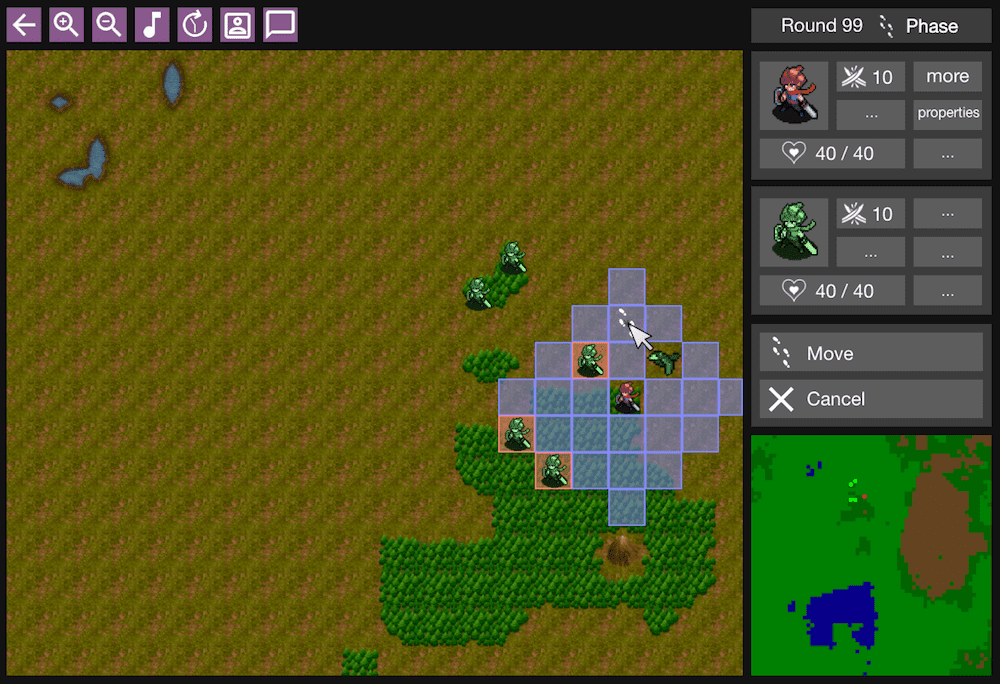
\includegraphics[width=0.8\textwidth]{images/mockUps/ConfirmMove.png}
                    	\caption{MockUp: Bewegen best"atigen (Phase 1)}
                    	\label{Move}
                    \end{figure}
	                \begin{figure}[H] 
	                	\centering
	                	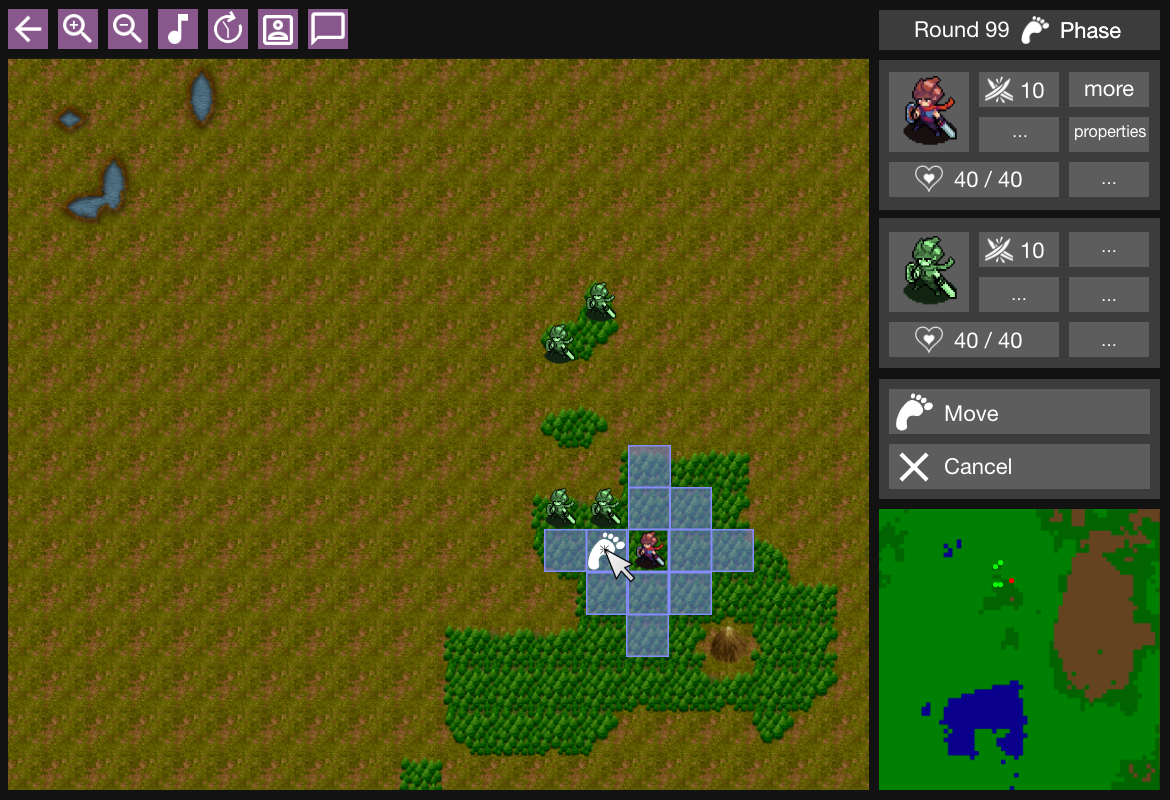
\includegraphics[width=0.8\textwidth]{images/mockUps/ConfirmMove2.png}
	                	\caption{MockUp: Bewegen best"atigen (Phase 3)}
	                	\label{Move2}
	                \end{figure}
			    \subsubsubsection{Einheit angreifen}
			        Nachdem der Nutzer in Phase 2 eine Einheit ausgew"ahlte und alle m"oglichen Angriffsziele angezeigt wurden, konnte er eine gegnerische Einheit neben ihm ausw"ahlen (insofern eine vorhanden war) und sie angreifen. \\
			        \begin{figure}[H] 
    				    \centering
    				    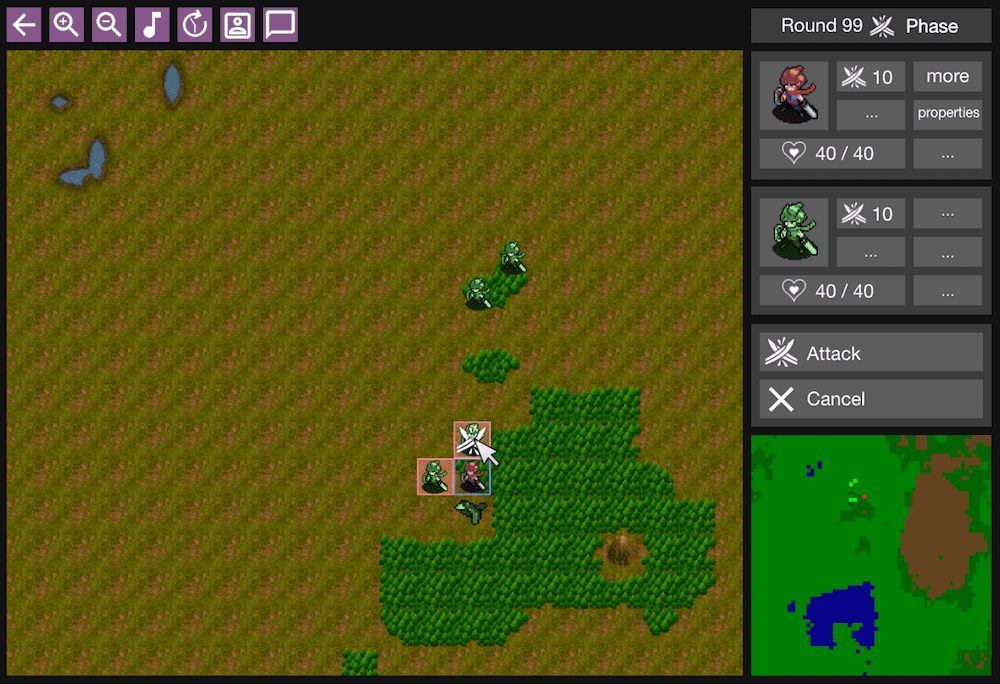
\includegraphics[width=0.8\textwidth]{images/mockUps/Attack.png}
    				    \caption{MockUp: Angreifen best"atigen}
    				    \label{Attack}
			        \end{figure}
		        	\ \\ War ein Gegner an der Reihe und der Server sendete eine angegriffene Einheit, dann sollten auch zuerst die m"oglichen Angriffsziele angezeigt werden und danach (kurz verz"ogert) sollte die Einheit angreifen. Sp"ater sollte dies auch noch "uber ein Box in der Sidebar best"atigt werden, um dem Nutzer die M"oglichkeit zu geben, seinen Angriff doch nicht durchzuf"uhren. Dabei sollte auf dem geklicktem Feld ein Icon angezeigt werden, bis der Nutzer die Aktion best"atigte oder abbruch (siehe Abbildung \ref{Attack}). War ein Gegner an der Reihe, wurde der Text und das Icon in der Box nicht angezeigt.
			    \subsubsubsection{Spielende}
			        Wenn ein Spieler verlor, da er keine Einheiten mehr hatte, sollte sich das Icon und der Name in seiner Playercard schwarz f"arben. Bei diesem Nutzer sollte ein Overlay angezeigt werden, in dem stand, dass er verloren hatte. Au"sserdem konnte er "uber das Overlay entscheiden, ob er sich zur"uck in die Lobby ging oder dem Spiel als Spectator beitrat (siehe Abbildung \ref{Game_Lost}). Wenn nur noch ein Spieler "ubrig war, gewann er das Spiel. Diesem Nutzer sollte auch ein Overlay angezeigt werden, durch das er zur"uck zur Lobby wechselte (siehe Abbildung \ref{Game_Won}). Bei anderen Nutzern, die sich im Spectatormodus befanden, sollte auch ein "ahnliches Overlay mit der gleichen Funktionalit"at angezeigt werden (siehe Abbildung \ref{Spactator_End}).
			        \begin{figure}[H] 
    				    \centering
    				    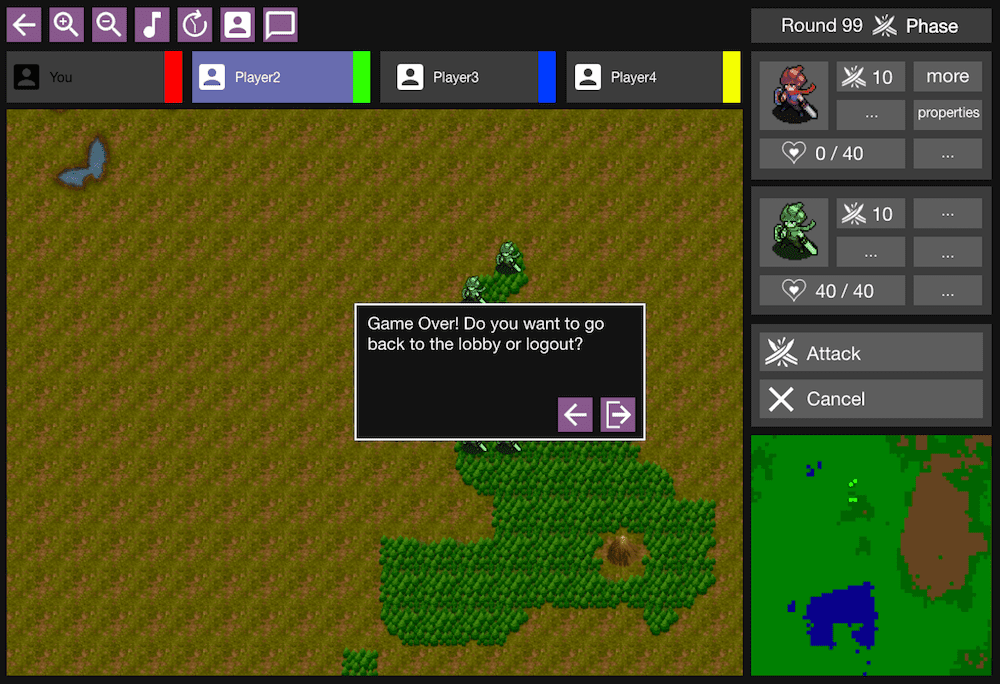
\includegraphics[width=0.8\textwidth]{images/mockUps/GameOver.png}
    				    \caption{MockUp: Spiel verloren}
    				    \label{Game_Lost}
			        \end{figure}
			        \begin{figure}[H] 
    				    \centering
    				    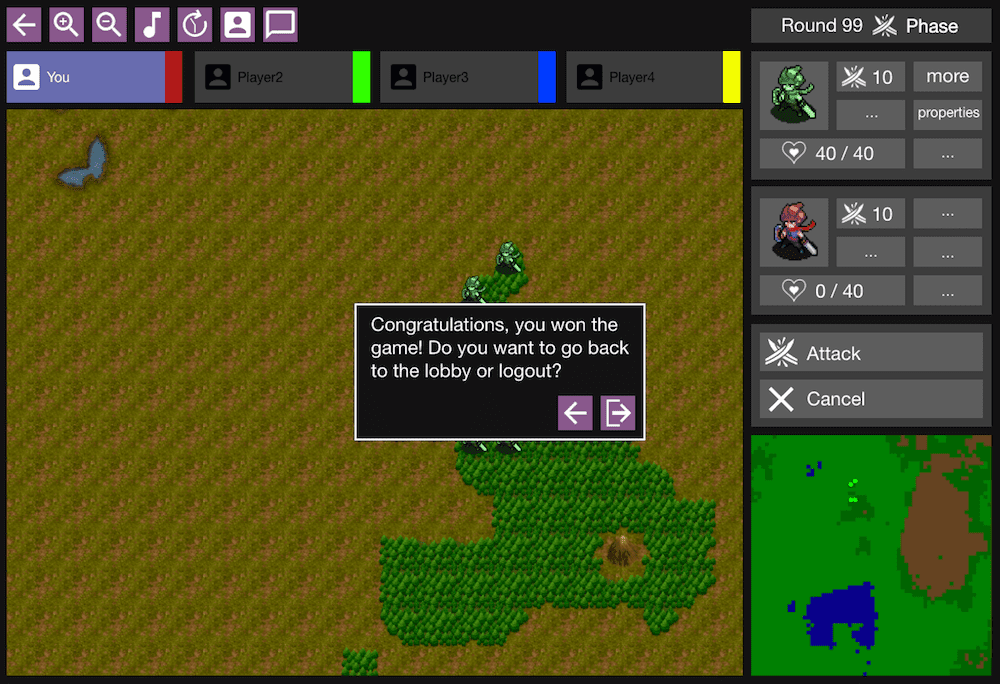
\includegraphics[width=0.8\textwidth]{images/mockUps/GameWon.png}
    				    \caption{MockUp: Spiel gewonnen}
    				    \label{Game_Won}
			        \end{figure}
			        \begin{figure}[H] 
    				    \centering
    				    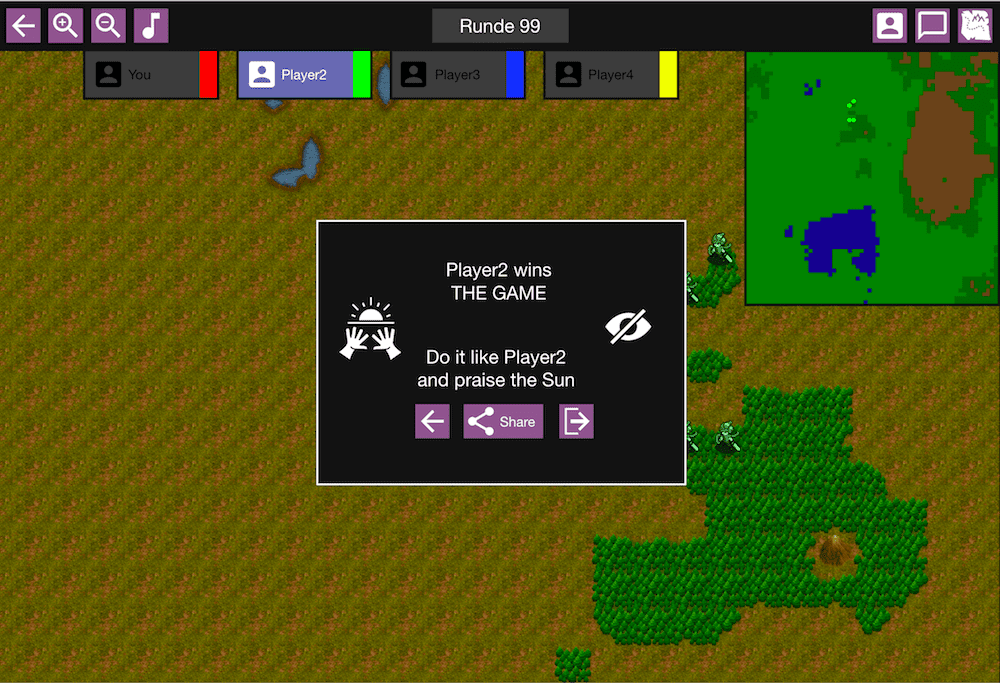
\includegraphics[width=0.8\textwidth]{images/mockUps/SpactatorEnd.png}
    				    \caption{MockUp: Beobachtungsmodus: Spiel vorbei}
    				    \label{Spactator_End}
			        \end{figure}
			    \subsubsubsection{Weitere Features}
			        Es sollte f"ur den Nutzer m"oglich sein, "uber einen Button die Phase beenden zu k"onnen und in die n"achste zu wechseln. Nach Beenden aller drei Phasen, musste auch die Runde beendet werden. Wenn ein Gegner an der Reihe war, musste der Phase beenden Button disabled sein. Beim Beenden der Phasen sollte immer ein Overlay angezeigt werden (siehe Abbildung \ref{Phase_End}). \\
			        \begin{figure}[H] 
    				    \centering
    				    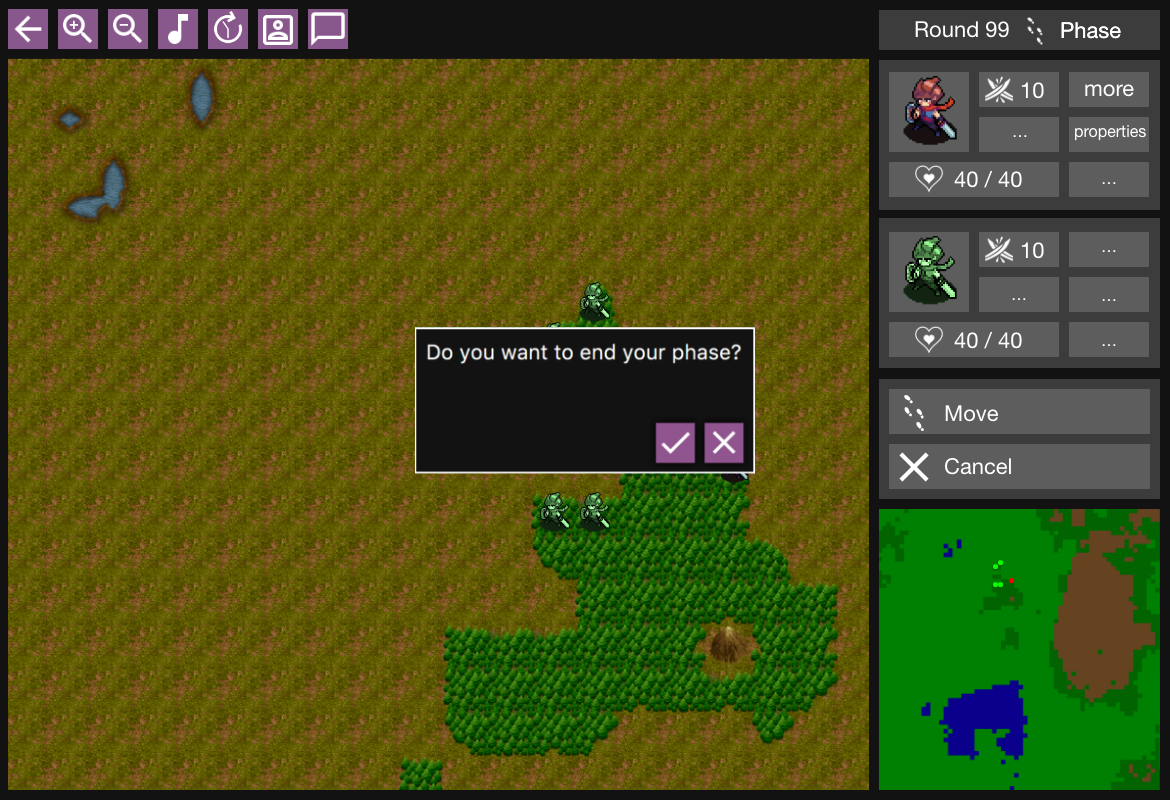
\includegraphics[width=0.8\textwidth]{images/mockUps/EndPhase.png}
    				    \caption{MockUp: Phase beenden}
    				    \label{Phase_End}
			        \end{figure}
			        \ \\ Es gab ein weiteres Feature, bei dem der Nutzer "uber eine Einheit hovern konnte, und je nachdem "uber welche Einheit der Nutzer hoverte, aktualisierten sich alle Properties und das Bild der gehoverten Einheit in der Sidebar. Die Einheiten des Spielers, der an der Reihe war, sollten in der oberen Box der Sidebar angezeigt werden. Die Einheiten der restlichen Spieler, die nicht an der Reihe waren, sollten in der unteren Box angezeigt werden. Zu Beginn jeder neuen Runde und sollten die beiden Boxen immer wieder leer sein und sich erst wieder f"ullen, wenn "uber eine EInheit gehovert bzw. wenn eine Aktion mit einer Einheit ausgef"uhrt wurde.
		\subsection{Domain Stories}
		    Domain Stories wurden einmal zum Ready geben f"ur den Waiting Room und einmal f"ur das Bewegen von Einheiten Ingame angefertigt. \\
		    TODO: Bilder einpflegen und beschreiben?
		    \ \\ Die Domain Stories wurden vor dem Release der Serverdokumentation f"ur das Kundentreffen erstellt. Deswegen zeigen sie leichte Abweichungen vom tats"achlichen Verhalten des Servers. Zum Beispiel sendet der Server Spiel starten erst, wenn irgendein Spieler den Befehl zum Spiel starten an den Server schickt, nachdem alle eine Ready gegeben haben. Wir nahmen an, dass der Server automatisch das Spiel startet, nachdem alle ready sind. Unsere Move Story trifft teilweise den Server. Der Unterschied zu unserer Story ist, dass wir vorher nicht davon ausgingen, dass eine Runde des Spielers in die drei Phasen unterteilt ist. Deswegen zeigt unsere Story auf dem MockUp oben rechts schon die bewegte Einheit, mit der jetzt eigentlich angegriffen werden sollte. Da dies vom Server her nicht funktioniert, m"ussen wir dies auf die drei Phasen unterteilen.
	\newpage
	\section{Sprint \RN{5}}
	    Der f"unfte Sprint erstreckte sich "uber dem Zeitraum vom 8.7.2019 bis zum 21.7.2019. Es wurden 116 Storypoints f"ur alle User Stories gesch"atzt.
	    \subsection{Sprintziel} \label{Sprintgoal_5}
	        Es sollte nach dem f"unften Sprint m"oglich sein:
	        \begin{itemize}
	            \item Einem Spiel beizutreten
	            \item Die Einheiten auf dem Spielfeld und der Minikarte zu sehen
	            \item Einheiten auszuw"ahlen, zu bewegen und anzugreifen
	            \item Den Spielstatus zu sehen und Phasen zu beenden
	        \end{itemize}
	        Falls die Entwicklung schneller als erwartet voranschreiten sollte, w"urden der Ingamechat und das Spielende noch implementiert werden. Sollten alle Ziele abgeschlossen werden, w"urden "uber 80 Storypoints abgearbeitet werden, was bei vier Entwicklern als ein guter Fortschritt gewertet werden k"onnte.
	    \subsection{User Stories} \label{User_Stories_5}
	        Die User Stories, die vom Product Owner erstellt wurden, sind wie gefolgt aufgebaut: Dem Titel kann entnommen werden zu welcher Szene die Story geh"ort. Anschlie"ssend werden die Story Points und der zugeteilte Entwickler genannt. Danach folgt das Ziel und die Story selbst. Das Ziel fasst die Subtasks, die der Scrum Master erstellt hat, zusammen.
	        \subsubsection{Waiting Room - Spielbeitritt anpassen}
	            \paragraph{Zuteilung}
	                Diese User Story wurde auf 5 Storypoints gesch\"atzt und an Omar Sood zugeteilt.
	            \paragraph{Ziel}
	                Der Spielbeitritt sollte an die Server\"anderungen angepasst werden. Das Ausw\"ahlen einer Armee sollte dem Server ein Bereit-Signal senden und das Spiel sollte starten, sobald alle Spieler bereit sind.
	            \paragraph{Story}
	                Karli befindet sich in der Wartreraumszene. Alle anderen Spieler sind bereit. Karli w"ahlt eine Armee aus. Da nun alle Spieler bereit sind, startet das Spiel (und es findet ein Szenenwechsel statt).
	            TODO: Verbindung zur Domain Story
            \subsubsection{Ingame - Spielfeld}
	            \paragraph{Zuteilung}
	                Diese User Story wurde auf 13 Storypoints gesch\"atzt und an Georg Siebert zugeteilt.
	            \paragraph{Ziel}
			   		Das Spielfeld sollte die Einheiten anzeigen. Jedes Feld musste anklickbar sein.
	            \paragraph{Story}
	                Karli befindet sich in der Ingameszene. Karli sieht die Einheiten auf dem Spielfeld. Karli klickt auf ein Feld (einer Einheit). Das Feld wird ausgew"ahlt.
	        \subsubsection{Ingame - Phase beenden}
	            \paragraph{Zuteilung}
	                Diese User Story wurde auf 3 Storypoints gesch\"atzt und an Juri Lozowoj zugeteilt.
	            \paragraph{Ziel}
	                Es sollte einen Button geben, welcher bei Bet\"atigung die aktuelle Phase beendete. Dies sollte nur m\"oglich sein, wenn der Nutzer auch seine Phase beenden konnte, da er an der Reihe war.
	            \paragraph{Story}
	                Karli befindet sich in der Ingameszene. Karli klickt auf den Phase-Beenden Button (siehe Mockup). Die Phase wird beendet und die n"achste tritt ein (bzw. der n"achste Spieler ist an der Reihe).
            \subsubsection{Ingame - Einheit ausw\"ahlen}
	            \paragraph{Zuteilung}
	                Diese User Story wurde auf 13 Storypoints gesch\"atzt und an Juri Lozowoj zugeteilt.
	            \paragraph{Ziel}
	                Durch Anklicken einer Einheit sollte diese Ausgew\"ahlt werden. Danach musste die Bewegungs- und Angriffsreichweite sichtbar sein, je nachdem in welcher Phase der Nutzer sich befand.
	            \paragraph{Story}
	                Karli befindet sich in der Ingameszene. Karli�w"ahlt eine Einheit durch Klicken auf ihre Graphik aus. G"ultige Bewegungsziele werden blau und g"ultige Angriffsziele rot markiert (siehe Mockups).
            \subsubsection{Ingame - Einheit bewegen}
	            \paragraph{Zuteilung}
	                Diese User Story wurde auf 13 Storypoints gesch\"atzt und an Omar Sood zugeteilt.
	            \paragraph{Ziel}
	                F\"ur die Bewegung einer Einheit sollte der k\"urzeste Pfad zum Zielfeld berechnet werden. Anschlie{\ss}end musste eine Nachricht an den Server gesendet und dessen Antwort korrekt verarbeitet werden.
	            \paragraph{Story}
	                Karli befindet sich in der Ingameszene. Karli w"ahlt eine Einheit aus, die Karli bewegen m"ochte. Karli klickt auf ein Feld in Bewegungsreichweite. Die Einheit wird bewegt.
	            TODO: Verbindung zur Domain Story
            \subsubsection{Ingame - Einheit angreifen}
	            \paragraph{Zuteilung}
	                Diese User Story wurde auf 5 Storypoints gesch\"atzt und an Omar Sood zugeteilt.
	            \paragraph{Ziel}
	                Es sollte m\"oglich sein, gegnerische Einheiten anzugreifen. Entsprechende Nachrichten sollten an den Server gesendet und dessen Antworten korrekt verarbeitet werden.
	            \paragraph{Story}
	                Karli befindet sich in der Ingameszene. Karli w"ahlt eine Einheit aus. Karli sieht alle Felder mit Einheiten in Rot, die angegriffen werden k"onnen. Karli w"ahlt eine gegnerische Einheit auf diesen Feldern aus. Die Einheit wird angegriffen.
            \subsubsection{Ingame - Spielstatus anzeigen}
	            \paragraph{Zuteilung}
	                Diese User Story wurde auf 8 Storypoints gesch\"atzt und an Tobias Klipp zugeteilt.
	            \paragraph{Ziel}
	                Es sollte einen Button zum Ein- und Ausblenden der Spielerinformationen implementiert werden. Der aktive Spieler sollte hervorgehoben werden.
	            \paragraph{Story}
	                Karli befindet sich in der Ingameszene. Karli sieht eine Runden- und Phasenanzeige. Karli klickt auf den Spieler-Anzeigen Button. Die Anzeige der Spieler wird eingeblendet (siehe Mockup). Der aktive Spieler ist hervorgehoben (in der selected-Color siehe Stylesheet bzw. MockUp).
            \subsubsection{Ingame - Minikarte anzeigen}
	            \paragraph{Zuteilung}
	                Diese User Story wurde auf 8 Storypoints gesch\"atzt und an Georg Siebert zugeteilt.
	            \paragraph{Ziel}
	                Es sollte eine Minikarte implementiert werden, die \"uber einen Button ein- und ausblendbar werden konnte.
	            \paragraph{Story}
	                Karli befindet sich in der Ingameszene. In der rechten oberen Ecke sieht Karli die Minikarte, welche neben dem Terrain auch alle Einheiten anzeigt. Karli dr"uckt den Minikarte Button. Die Minikarte wird ausgeblendet.
            \subsubsection{Ingame - Chatintegration}
	            \paragraph{Zuteilung}
	                Diese User Story wurde auf 13 Storypoints gesch\"atzt und an Tobias Klipp zugeteilt.
	            \paragraph{Ziel}
	                Es sollte einen Button zum Ein- und Ausblenden des Chats implementiert werden.
	            \paragraph{Story}
	                Karli befindet sich in der Ingameszene. Karli dr"uckt den Chat-Einblenden Button. Der Chat wird angezeigt. Karli schreibt eine Nachricht. Die Nachricht wird im Chat f"ur alle Spieler im Spiel angezeigt. Bob schreibt eine Nachricht. Karli kann Bobs Nachricht lesen.
            \subsubsection{Ingame - Game Over}
	            \paragraph{Zuteilung}
	                Diese User Story wurde auf 2 Storypoints gesch\"atzt und an Tobias Klipp zugeteilt.
	            \paragraph{Ziel}
	                Wenn der Nutzer verloren hatte, sollte ein Overlay angezeigt werden. Auf diesem konnte er in die Lobby wechseln oder dem Spiel zuschauen.
	            \paragraph{Story}
	                Karli befindet sich in der Ingameszene. Karlis Playerkarte f�rbt sich schwarz (Name und Icon). Karli sieht ein Overlay aufgehen, auf welchem Karli gefragt wird, ob Karli das Spiel weiter betrachten m�chte. Karli dr�ckt den Cancel Button. Karli wechselt in die Lobby.
            \subsubsection{Ingame - Game Won}
	            \paragraph{Zuteilung}
	                Diese User Story wurde auf 2 Storypoints gesch\"atzt und an Tobias Klipp zugeteilt.
	            \paragraph{Ziel}
                      Wenn der Nutzer gewann, sollte ein Overlay angezeigt werden, das ihn in die Lobby wechseln lie"ss.
	            \paragraph{Story}
	                Karli befindet sich in der Ingameszene. Karli besiegt die letzte gegnerische Einheit. Karli sieht ein Overlay aufgehen (siehe MockUp). Karli wechselt in die Lobby.
             \subsubsection{Ingame - Spectator Over}
             	\paragraph{Zuteilung}
             		Diese User Story wurde auf 2 Storypoints gesch\"atzt und an Tobias Klipp zugeteilt.
             	\paragraph{Ziel}
             		Wenn das Spiel vorbei war, sollte dem Nutzer ein Overlay angezeigt werden, durch das er in die Lobby wechselte.
             	\paragraph{Story}
             		Karli befindet sich in der Ingameszene. Bob besiegt die letzte gegnerische Einheit. Karli sieht ein Overlay aufgehen (siehe MockUp). Karli wechselt in die Lobby.
            \subsubsection{Lobby - Spectating}
	            \paragraph{Zuteilung}
	                Diese User Story wurde auf 5 Storypoints gesch\"atzt und an Juri Lozowoj zugeteilt.
	            \paragraph{Ziel}
	                Es sollte ein Button hinzugef\"ugt werden, der einen Spielbeitritt als Beobachter erm\"oglichte.
	            \paragraph{Story}
	                Karli befindet sich in der Lobbyszene.  Karli sieht die Spielliste und m"ochte dieses mal nicht selbst spielen. Karli dr"uckt auf den Spactator-Button. Karli wird in den Warteraumszene weitergeleitet.
            \subsubsection{Ingame - Spectating}
	            \paragraph{Zuteilung}
	                Diese User Story wurde auf 13 Storypoints gesch\"atzt und an Juri Lozowoj zugeteilt.
	            \paragraph{Ziel}
	                Das Spiel sollte so angepasst werden, dass ein Zuschauer weder mit dem Spielfeld interagieren, noch Chatnachrichten schreiben konnte.
	            \paragraph{Story}
	                Karli befindet sich in der Ingameszene. Karli versucht etwas in den Chat zu schreiben. Karli versucht Aktionen mit den Einheiten auszuf�hren. Karlis Aktionen funktionieren nicht. Karli merkt aber, dass alles andere funktioniert, holt Popcorn und genie�t das Spiel.
            \subsubsection{Ingame - Einheiteninformationen}
	            \paragraph{Zuteilung}
	                Diese User Story wurde auf 8 Storypoints gesch\"atzt und an Georg Siebert zugeteilt.
	            \paragraph{Ziel}
	                Bewegte der Nuzter die Maus \"uber eine Einheit, sollten alle verf\"ugbaren Informationen dieser Einheit in einem Kontextmen"u angezeigt werden.
	            \paragraph{Story}
	                Karli befindet sich in der Ingameszene. Karli f"ahrt mit seinem Mouse-Courser "uber eine Einheit. Alle wichtigen Informationen �ber die Einheit werden in einem Kontextmen"u angezeigt.
            \subsubsection{Ingame - Musiksteuerung}
	            \paragraph{Zuteilung}
	                Diese User Story wurde auf 3 Storypoints gesch\"atzt und an Omar Sood zugeteilt.
	            \paragraph{Ziel}
	                Es sollte ein Musik Button hinzugef\"ugt werden, mit dem sich die Musik genauso bedienen lie"ss wie in den restlichen Szenen.
	            \paragraph{Story}
	                Karli befindet sich in der Ingameszene und die Musik spielt. Karli klickt auf den Musik Button (siehe Mockup). Die Musik wird ausgeschaltet.
        \subsection{Tasks} \label{Tasks_5}
            Die Tasks wurden vom Scrum Master erstellt und sind nicht aus Nutzersicht beschreibbar, da sie nur technische Aufgaben waren. Aus diesem Grund unterschieden sich Tasks nur in einer Sache von User Stories. Sie hatten keine Story.
            \subsubsection{Servernachrichten}
            	\paragraph{Zuteilung}
            		Diese Task wurde auf 8 Zeitstunden gesch\"atzt und an Omar Sood zugeteilt.
            	\paragraph{Ziel}
            		Der Entwickler sollte alle restlichen Servernachrichten abfangen, die in keiner User Story ber\"ucksichtig wurden. Dazu geh\"orten unter anderem \"Anderungen des Datenmodells, welche durch Aktionen der Gegenspieler anfielen.
            \subsubsection{Einheiteninformationen im Datenmodell}
            	\paragraph{Zuteilung}
            		Diese Task wurde auf 5 Zeitstunden gesch\"atzt und an Tobias Klipp zugeteilt.
            	\paragraph{Ziel}
            		Der Entwickler sollte die Enums UnitType und UnitTypeInfo zu einer Enum zusammenf\"ugen und musste darauf achten, dass alle Funktionalit\"aten erhalten blieben.
        \subsection{Zeit"ubersicht}
        	Diese \"Ubersicht zeigt alle Stories, welche im Rahmen der Ziele bearbeitet werden sollten. Wie zu erkennen ist, wurden nicht alle Stories abgeschlossen. Es wurden jedoch schon umfangreichere Grundlagen f\"ur Features des sechsten Sprints gelegt.
        	\begin{longtable}[H]{p{6cm} c c c c }
        			\label{Time_1}
       				\textbf{User Story} & \textbf{Soll Zeit} & \textbf{Ist Zeit} & \textbf{Noch Zeit} & \textbf{Entwickler} \\
       				\toprule
       				\endhead
       				Waiting Room - Spielbeitritt anpassen & 5 h & 13 h 9 min & - & Omar Sood\\
       				Ingame - Spielfeld & 13 h & 8 h 22 min & - & Georg Siebert\\
       				Ingame - Phase beenden & 3 h & 15 h 20 min & - & Juri Lozowoj \\
       				Ingame - Einheit ausw"ahlen & 13 h & 8 h 46 min & 4h 14 min & Juri Lozowoj \\
       				Ingame - Einheit bewegen & 13 h & 11 h 19 min & 35 min & Omar Sood \\
       				Ingame - Einheit angreifen & 5 h & - & 5 h & Omar Sood \\
       				Ingame - Spielstatus anzeigen & 8 h & 18 h 45 min & - & Tobias Klipp \\
       				Ingame - Minikarte anzeigen & 8 h & 8 h 25 min & 4 h & Georg Siebert \\
       				Ingame - Chatintegration & 13 h & - & 13 h & Tobias Klipp \\
       				Ingame - Game Over & 2 h & - & 2 h & Tobias Klipp \\
       				Ingame - Game Won & 2 h & - & 2 h & Tobias Klipp \\
        			\caption{Zeit"ubersicht f"unfter Sprint}
        	\end{longtable}
        \subsection{Analyse}
        	Der f\"unfte Sprint endete am 21.7.2019. Das Team schaffte 29 der 116 gesch\"atzten Storypoints.
        	\subsubsection{Burndown}
        		Wie im Burndown-Diagramm zu sehen ist, wurden diesen Sprint nur vier Stories mit einem Umfang von 29 Storypoints abgeschlossen (siehe Kapitel \ref{done_stories_5}). Wie Tabelle \ref{Time_1} zeigt, betrug die Arbeitszeit trotzdem 84 Stunden. Die Hauptursache war die Untersch\"atzung der Aufgabenumf\"ange, wodurch mehrere begonnene Stories in diesem Sprint nicht mehr abgeschlossen werden konnten und andere deutlich mehr Zeit als erwartet in Anspruch nahmen. Zudem f\"uhrte die in diesem Release h\"ohere Anzahl an blockierenden und relatierten Tasks zu einer insgesamt langsamereren Entwicklung, da sich die Entwickler h\"aufig miteiander absprechen mussten.
	        	\begin{figure}[H] 
	        		\centering
	        		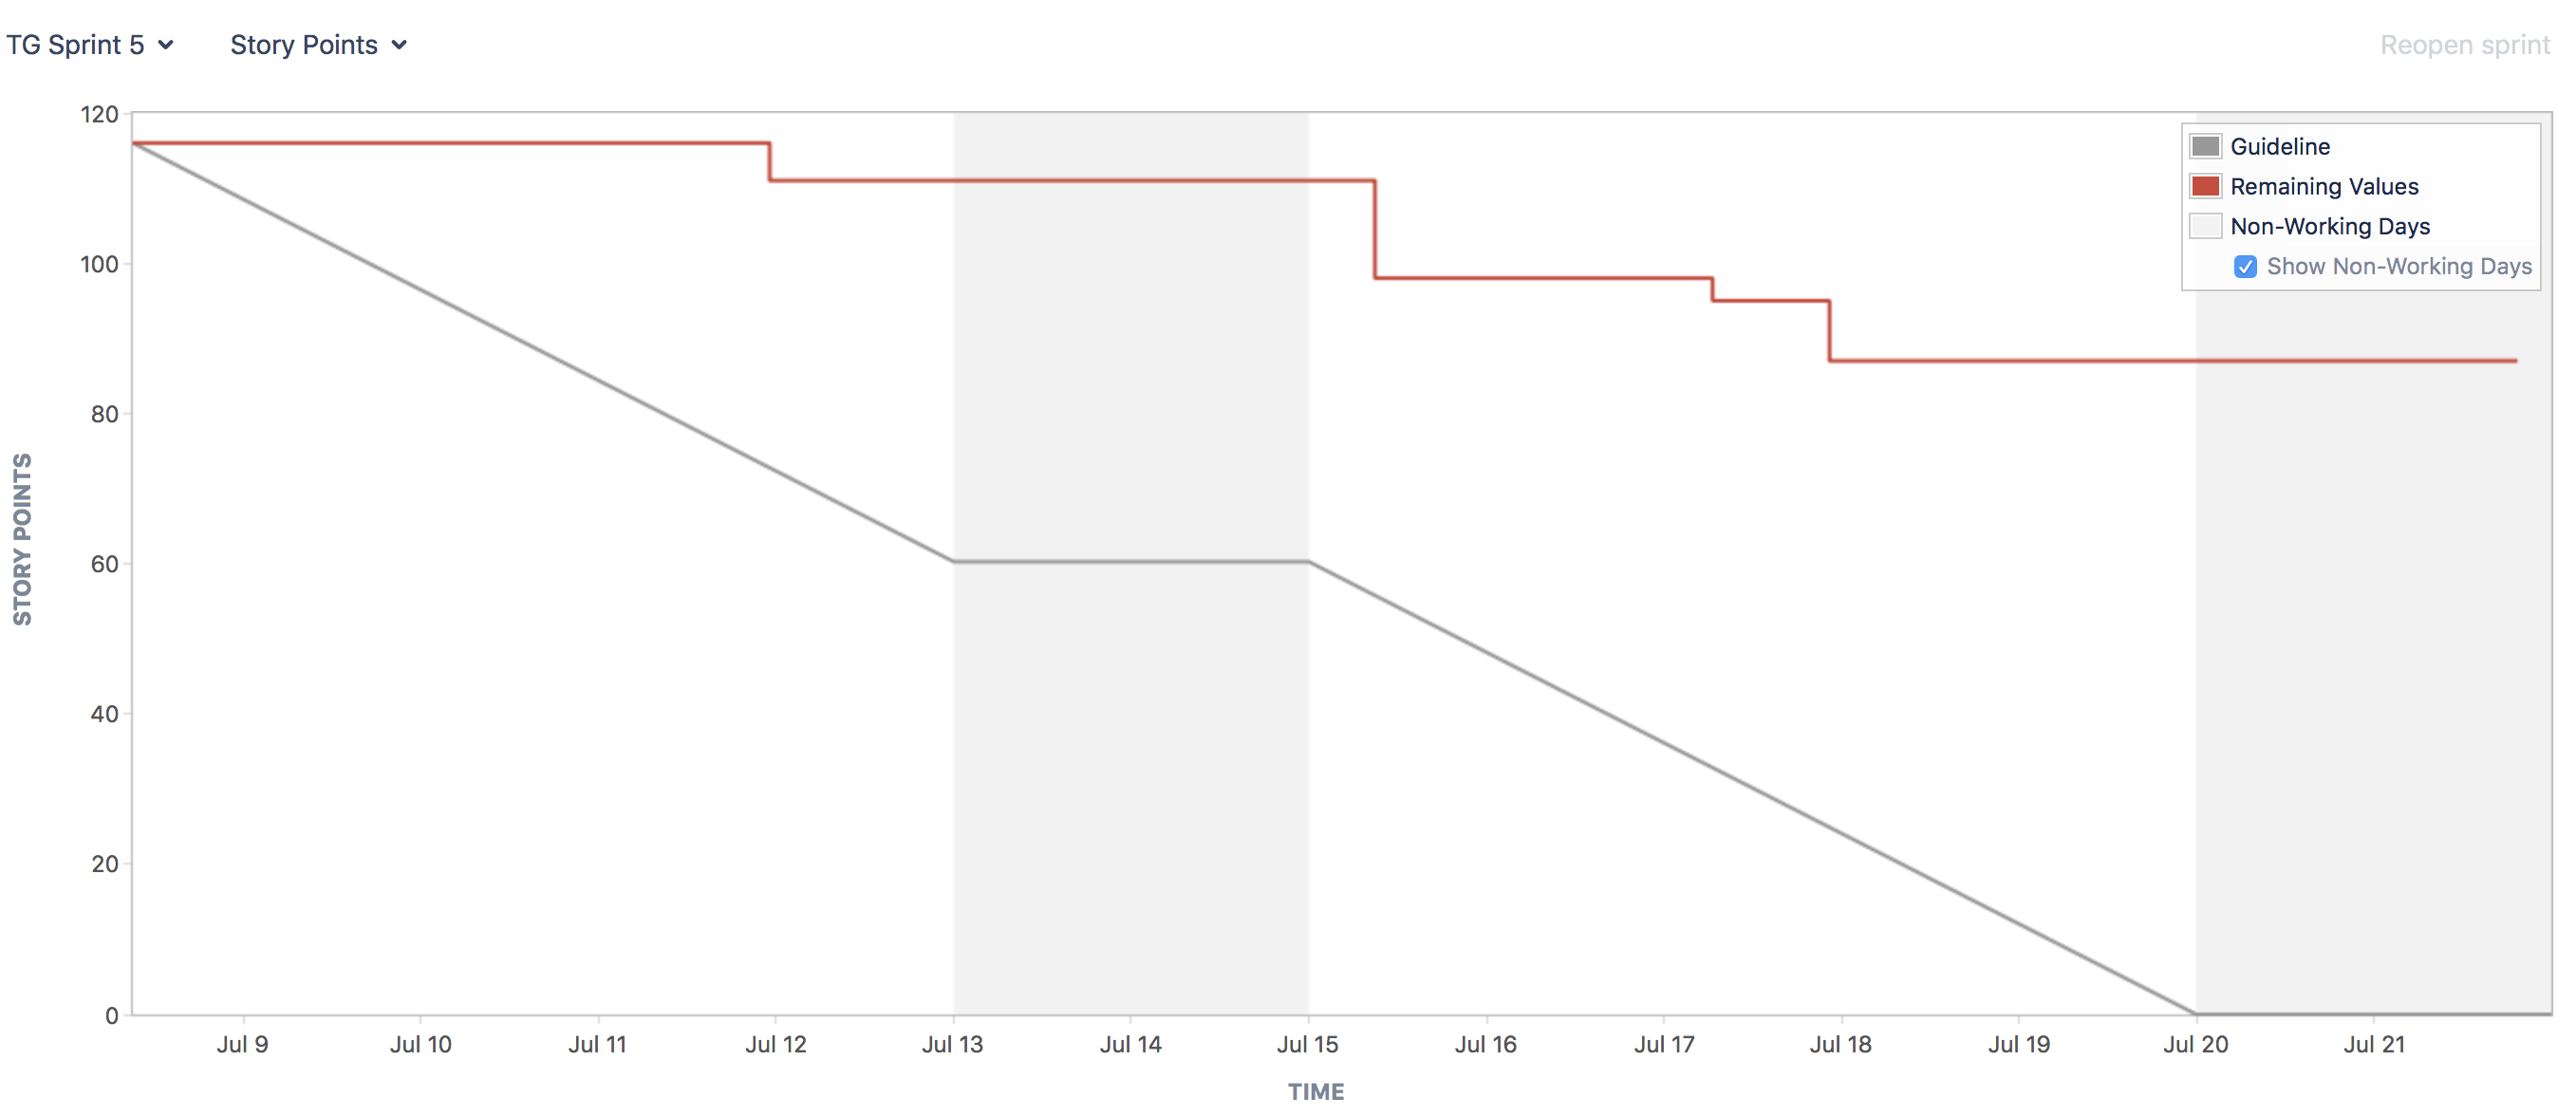
\includegraphics[width=\textwidth]{images/sprintV/burndown.png}
	        		\caption{Sprint \RN{5}: Burndown Diagramm}
	        		\label{Burndown_5}
	        	\end{figure} 
        	\subsubsection{Abgeschlossene Stories} \label{done_stories_5}
        		Es wurden bisher vier Stories abgeschlossen (siehe Abbildung \ref{Done_5}). Dies war weniger als erwartet, aber aufgrund komplexer Aufgaben nicht zu vermeiden. Im Nachhinein wird es nun eine genauere Beschreibung der abgeschlossenen Stories geben.
        		\begin{figure}[H] 
        			\centering
        			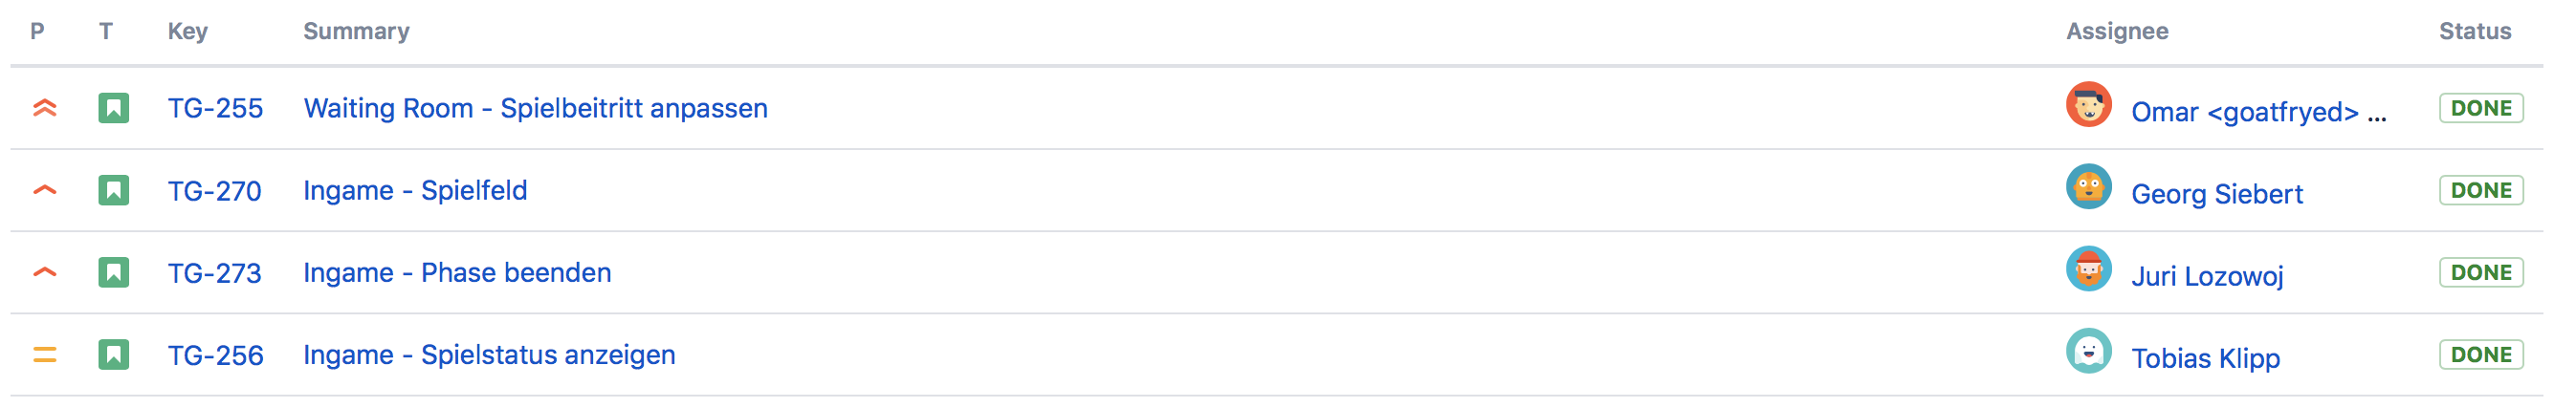
\includegraphics[width=\textwidth]{images/sprintV/done.png}
        			\caption{Sprint \RN{5}: Abgeschlossene Stories}
        			\label{Done_5}
        		\end{figure}
        		\subsubsubsection{Waiting Room - Spielbeitritt anpassen}
	        		\paragraph{Verlauf}
	        			TODO: Schreiben
	        		\paragraph{Ergebnis}
	        			TODO: Schreiben
       			\subsubsubsection{Ingame - Spielfeld}
	       			\paragraph{Verlauf}
	       				TODO: Schreiben
	       			\paragraph{Ergebnis}
	       				TODO: Schreiben
    			\subsubsubsection{Ingame - Phase beenden}
    				\paragraph{Verlauf}
    					TODO: Schreiben
    				\paragraph{Ergebnis}
    					TODO: Schreiben
    			\subsubsubsection{Ingame - Spielstatus anzeigen}
    				\paragraph{Verlauf}
    					TODO: Schreiben
    				\paragraph{Ergebnis}
    					TODO: Schreiben
        	\subsubsection{Angefangene Stories}
        		Wie bereits in der Analyse des Burndowns erw\"ahnt wurde, wurden drei bereits begonnene Stories zum Ende des Sprints noch nicht abgeschlossen. Im kommenden Abschnitt wird es einen \"Uberblick geben, wie weit diese bearbeitet wurden.
        		\subsubsubsection{Ingame - Einheit ausw"ahlen}
        			\paragraph{Verlauf}
	        			TODO: Schreiben
        			\paragraph{Stand}
        				TODO: Schreiben
        		\subsubsubsection{Ingame - Einheit bewegen}
        			\paragraph{Verlauf}
        				TODO: Schreiben
        			\paragraph{Stand}
        				TODO: Schreiben
        		\subsubsubsection{Ingame - Minikarte anzeigen}
        			\paragraph{Verlauf}
        				TODO: Schreiben
        			\paragraph{Stand}
        				TODO: Schreiben
        	\subsubsection{Nicht abgeschlossene Stories/Tasks}
        		Des Weiteren wurden neben den drei bereits angefangenen Stories noch weitere elf Stories beziehungsweise Tasks aufgrund von Zeitgr\"unden nicht angefangen und abgeschlossen (siehe Abbildung \ref{To_Do_5}). Diese Aufgaben waren nicht optional und sollten von unserem Team im n\"achsten Sprint bew\"altigt werden.
        		\begin{figure}[H] 
        			\centering
        			\includegraphics[width=\textwidth]{images/sprintV/toDo.png}
        			\caption{Sprint \RN{5}: Nicht Abgeschlossene Stories/Tasks}
        			\label{To_Do_5}
        		\end{figure}
        	\subsubsection{Fazit}
        		Die Ziele des Sprints wurden verfehlt. Um die Mindestanforderungen zu erreichen, m"usste das Entwicklerteam seine Produktivit\"at im sechsten Sprint deutlich steigern. Da die C0 Abdeckung (siehe Abbildung \ref{Coverage_5}) zum Ende des f\"unften Sprints bereits 79\% betrug, gab es bei der Qualit\"atssicherung keine Defizite.
        		\begin{figure}[H] 
        			\centering
        			\includegraphics[width=0.8\textwidth]{images/sprintV/coverage.png}
        			\caption{Sprint \RN{5}: C0 Testabdeckung (Siehe Line, \%)}
        			\label{Coverage_5}
        		\end{figure} 
    \newpage
    \section{Sprint \RN{6}}
    	Der sechste Sprint erstreckte sich \"uber dem Zeitraum vom 22.7.2019 bis zum 4.8.2019. Er umfasst 87 Storypoints.
    	\subsection{Sprintziel}
    		Es sollte nach dem sechsten Sprint m\"oglich sein:
    		\begin{itemize}
    			\item Alle Features aus dem Sprint \RN{5} (siehe Kapitel \ref{Sprintgoal_5}) zu verwenden
    			\item Einen Ingame Chat zu benutzen
    			\item Verschiedene Overlays beim Spielende zu sehen
    			\item Einem Spiel als Beobachter beizutreten
    			\item Einheiteninformationen in einer Sidebar einzusehen
    			\item Die Musik auch im Spiel ein- und auszuschalten
    		\end{itemize}
    		F\"ur den Fall, dass die Mindestanforderungen vor Ende des Sprints abgeschlossen werden sollten, sollte eine Sidebar zum Spielfeld hinzugef\"ugt werden. Diese sollte es erm\"oglichen Aktionen, wie Bewegen oder Angreifen, zu best\"atigen und abzubrechen. Falls das Team die Umsetzung der oben genannten Features schaffen w"urde, w"aren die Mindestanforderungen jedoch bereits erf\"ullt.
    	\subsection{Ge\"anderte User Stories vom Sprint \RN{5}}
    		Die folgenden Stories des f\"unften Sprints wurden aktualisiert, da sich ihre Mockups "anderten.
    		\subsubsection{Ingame - Minikarte anzeigen}
    			 \paragraph{Zuteilung}
    				Diese User Story wurde auf 8 Storypoints gesch\"atzt und an Georg Siebert zugeteilt.
    			\paragraph{Ge\"andertes Ziel}
    				Es sollte eine Minikarte implementiert werden. \"Uber die Minikarte sollte es m\"oglich sein, den Sichtbereich zu wechseln.
    			\paragraph{Ge\"anderte Story}
    				Karli befindet sich in der Ingameszene. In der rechten unteren Ecke sieht Karli die Minikarte, welche neben dem Terrain auch alle Einheiten anzeigt. Karli dr"uckt auf eine Stelle in der Minikarte. Der Sichtbereich "andert sich zu dieser Stelle.
   			\subsubsection{Ingame - Einheiteninformationen}
   				\paragraph{Zuteilung}
   					Diese User Story wurde auf 8 Storypoints gesch\"atzt und an Georg Siebert zugeteilt.
   				\paragraph{Ge\"andertes Ziel}
   					Bewegte der Nutzer die Maus \ "uber eine Einheit, sollten alle verf\"ugbaren Informationen dieser Einheit in einer Sidebar angezeigt werden.
   				\paragraph{Ge\"anderte Story}
   					Karli befindet sich in der Ingameszene. Karli f"ahrt mit Karlis Mouse-Courser "uber eine Einheit. Alle wichtigen Informationen "uber die Einheit werden in der Sidebar angezeigt (siehe MockUps).
   		\subsection{\"Ubernommene User Stories aus Sprint \RN{5}}
   			Weiterhin gab es auch User Stories aus dem f\"unften Sprint, welche noch nicht abgeschlossen wurden. Diese wurden mit in den sechsten Sprint \"ubernommen. Es folgt eine Liste dieser Stories:
   			\begin{itemize}
   				\item Ingame - Einheit ausw\"ahlen (angefangen in Sprint \RN{5})
   				\item Ingame - Einheit bewegen (angefangen in Sprint \RN{5})
   				\item Ingame - Einheit angreifen
   				\item Ingame - Spielstatus anzeigen (angefangen in Sprint \RN{5})
   				\item Ingame - Minikarte anzeigen (angefangen in Sprint \RN{5})
   				\item Ingame - Chatintegration
   				\item Ingame - Game Over
   				\item Ingame - Game Won
   				\item Ingame - Spectator Over
   				\item Lobby - Spectating
   				\item Ingame - Spectating
   				\item Ingame - Einheiteninformationen
   				\item Ingame - Musiksteuerung
   			\end{itemize}
   			Eine genauere Beschreibung zu jeder Story befindet sich im Kapitel \ref{User_Stories_5}.
   		\subsection{User Stories}
   			Im sechsten Sprint wurden weitere User Stories vom Product Owner erstellt.
   			\subsubsection{Ingame - Einheit bewegen nach Bewegung}
   				\paragraph{Zuteilung}
   					Diese User Story wurde auf 5 Storypoints gesch\"atzt und an Omar Sood zugeteilt.
   				\paragraph{Ziel}
   					Nachdem der Nutzer eine Einheit bewegte, sollte diese erneut ausgew�hlt sein, falls sie noch verbleibende Bewegungspunkte besa"ss.
   				\paragraph{Story}
   					Karli befindet sich in der Ingameszene. Karli klickt auf eine Einheit. Die Bewegungsreichweite wird angezeigt. Karli klickt auf ein Feld in Bewegungsreichweite. Die Einheit wird bewegt und bleibt weiterhin ausgew"ahlt, aber der blaue Bewegungsradius hat sich verkleinert. Karli bewegt die Einheit noch einmal auf ein weiteres Feld. Die Bewegungspunkte sind noch nicht aufgebraucht und die Einheit bleibt weiter ausgew"ahlt. Karli hat keine Lust mehr die Einheit zu bewegen und w"ahlt sie ab.
   		\subsection{Ge\"anderte Tasks vom Sprint \RN{5}}
   			Die folgenden Tasks des f\"unften Sprints wurden aktualisiert, da sich ihre Zuteilung "anderte.
   			\subsubsection{Einheiteninformationen im Datenmodell}
   				\paragraph{Ge"andete Zuteilung}
   					Diese Task wurde auf 5 Zeitstunden gesch\"atzt und an Omar Sood zugeteilt.
   				\paragraph{Ziel}
   					Der Entwickler sollte die Enums UnitType und UnitTypeInfo zu einer Enum zusammenf\"ugen und musste darauf achten, dass alle Funktionalit\"aten erhalten blieben.
    	\subsection{\"Ubernommene Tasks aus Sprint \RN{5}}
    		Weiterhin gab es auch Tasks aus dem f\"unften Sprint, welche noch nicht abgeschlossen wurden. Diese wurden mit in den sechsten Sprint \"ubernommen. Es folgt eine Liste dieser Tasks:
	    	\begin{itemize}
	    		\item Servernachrichten
	    		\item Einheiteninformationen im Datenmodell
	    	\end{itemize}
    		Eine genauere Beschreibung zu jeder Task befindet sich im Kapitel \ref{Tasks_5}.
   		\subsection{Tasks}
   			Im sechsten Sprint wurden weitere Tasks vom Scrum Master erstellt.
   			\subsubsection{Ingame - Best�tigungsbox in der Sidebar}
   				\paragraph{Zuteilung}
   					Diese Task wurde auf TODO Zeitstunden gesch"atzt und dan Georg Siebert zugeteilt.
				\paragraph{Ziel}
					Es musste eine Box in der Sidebar erstellt werden, die es m"oglich machte, Aktionen zu best"atigen oder abzubrechen (Die Funktionalit"aten sollten erst sp"ater in den untergeordneten User Stories erstellt werden). War der User nicht an der Reihe oder im Beobachtungsmodus, musste diese Box disabled werden. Beziehungsweise sollte dann auf den beiden Buttons der Text und das Icon nicht mehr sichtbar sein.
		\subsection{Bugs}
			Bugstasks zum Beheben von Problemen wurden vom Scrum Master erstellt, da im Verlauf der Entwicklung und beim Testen des Clients der ein oder andere Fehler aufkam.
			\subsubsection{Terminierung sicherstellen}
				\paragraph{Zuteilung}
					Dieser Bug sollte von Omar Sood behoben werden.
				\paragraph{Problem}
					Die Terminierung des GameEventSockets musste angepasst werden. Sie sollte nicht doppelt aufgerufen werden. Weiterhin sollte sie immer stattfinden, wenn der Nutzer die Anwendung schloss oder in die Lobby wechselte.
			\subsubsection{Ingame - Einheit mehrmals ausw�hlen}
				\paragraph{Zuteilung}
					Dieser Bug sollte von Juri Lozowoj behoben werden.
				\paragraph{Problem}
					Falls der Nutzer eine Einheit ausw�hlte, abw�hlte und dann wieder ausw�hlte, ohne vorher eine andere Einheit ausgew�hlt zu haben, wurde sie danach als Angriffs- bzw. Bewegungsziel farblich markiert. Dies sollte nicht stattfinden.
     \newpage	
    	\subsection{Zeit\"ubersicht}
    		TODO: Intro schreiben
    		\begin{longtable}[H]{p{6cm} c c c c }
    			\label{Time_2}
    			\textbf{User Story/Task} & \textbf{Soll Zeit} & \textbf{Ist Zeit} & \textbf{Noch Zeit} & \textbf{Entwickler} \\
    			\toprule
    			\endhead
    			Ingame - Einheit ausw\"ahlen & 13 h & 16 h 29 min & - & Juri Lozowoj \\
    			Ingame - Einheit bewegen & 13 h & 13 h 35 min & - & Omar Sood \\
    			Ingame - Einheit angreifen & 5 h & - & 5 h & Omar Sood \\
    			Ingame - Chatintegration & 13 h & 2 h & 11 h & Tobias Klipp \\
    			Ingame - Minikarte anzeigen & 8 h & 12 h 14 min & - & Georg Siebert \\
    			Lobby - Spectating & 5 h & - & 5 h & Juri Lozowoj \\
    			Ingame - Spectating & 13 h & - & 13 h & Juri Lozowoj \\
    			Ingame - Game Over & 2 h & - & 2 h & Tobias Klipp \\
    			Ingame - Game Won & 2 h & - & 2 h & Tobias Klipp \\
    			Ingame - Spectator Over & 2 h & - & 2 h & Tobias Klipp \\
    			Ingame - Einheiteninformationen & 8 h & 1 h & 7 h & Georg Siebert \\
    			Ingame - Spielstatus anzeigen & 8 h & 31 h 30 min & - & Tobias Klipp \\
    			Ingame - Musiksteuerung & 3 h & 20 min & - & Omar Sood \\
    			Ingame - Einheit bewegen nach Bewegung & 5 h & - & 5 h & Omar Sood \\
    			\midrule
    			Einheiteninformationen im Datenmodell & 5 h & 1 h 27 min & - & Omar Sood \\
    			Servernachrichten & 8 h & - & - & Omar Sood \\
    			Ingame - Best�tigungsbox in der Sidebar & ? h & - & - & Georg Siebert \\
    			\midrule
    			Terminierung sicherstellen & - & - & ? & Omar Sood \\
    			Ingame - Einheit mehrmals ausw�hlen & - & - & ? & Juri Lozowoj \\
    			\caption{Zeit\"ubersicht sechster Sprint}
    		\end{longtable}
    	\subsection{Analyse}
    		TODO: Intro schreiben
	    	\subsubsection{Burndown}
	    		TODO: Schreiben
	    	\subsubsection{Ausrei{\ss}er}
	    		TODO: Schreiben
	    	\subsubsection{Abgeschlossen}
	    		TODO: Schreiben
	    		\subsubsection{Angefangen}
	    		TODO: Schreiben
	    	\subsubsection{Nicht abgeschlossen}
	    		TODO: Schreiben
	    	\subsubsection{Entfernt}
	    		TODO: Schreiben
	    	\subsubsection{Fazit}
	    		TODO: Schreiben
	\newpage
	\section{Abschluss Release \RN{3}}
		TODO: Intro schreiben
		\subsection{Neue MockUps im Verlauf des Releases \RN{3}}
		TODO: Schreiben
		\subsection{Vergleich MockUps mit aktueller Implementation}
		TODO: Schreiben
	\newpage
	\section{Quellenangaben}
		\listoffigures
		\listoftables
\end{document}